\documentclass[mstat,12pt]{unswthesis}



%%%%%%%%%%%%%%%%%%%%%%%%%%%%%%%%%%%%%%%%%%%%%%%%%%%%%%%%%%%%%%%%%%
% 
% OK...Now we get to some actual input.  The first part sets up
% the title etc that will appear on the front page
%
%%%%%%%%%%%%%%%%%%%%%%%%%%%%%%%%%%%%%%%%%%%%%%%%%%%%%%%%%%%%%%%%%

\title{Capstone Project by Team What Watts\\[0.5cm]A Data Science
Approach to Forecast Electricity Consumption in Australia}

\authornameonly{(Nee) Jittinun Trairattanasirikul - (z5281789) (Ruhul)
Md Ruhul Amin Sarker - (z5275314) Peter Morian - (z5017159) James
Cleaver - (z5283034) }

\author{\Authornameonly}

\copyrightfalse
\figurespagefalse
\tablespagefalse

%%%%%%%%%%%%%%%%%%%%%%%%%%%%%%%%%%%%%%%%%%%%%%%%%%%%%%%%%%%%%%%%%
%
%  And now the document begins
%  The \beforepreface and \afterpreface commands puts the
%  contents page etc in
%
%%%%%%%%%%%%%%%%%%%%%%%%%%%%%%%%%%%%%%%%%%%%%%%%%%%%%%%%%%%%%%%%%%


%%%%%%%%%%%%%%%%%%%%%%%%%%%%%%%%%%%%%%%%%%%%%%%%%%%%%%%%%%%%%%%%%%%%%%%
%
%  A small sample UNSW Coursework Masters thesis file.
%  Any questions to Ian Doust i.doust@unsw.edu.au and/or Gery Geenens ggeenens@unsw.edu.au
%
%%%%%%%%%%%%%%%%%%%%%%%%%%%%%%%%%%%%%%%%%%%%%%%%%%%%%%%%%%%%%%%%%%%%%%%
%
%  The first part pulls in a UNSW Thesis class file.  This one is
%  slightly nonstandard and has been set up to do a couple of
%  things automatically
%
 
%%%%%%%%%%%%%%%%%
%% Precisely one of the next four lines should be uncommented.
%% Choose the one which matches your degree, uncomment it, and comment out the other two!
%\documentclass[mfin,12pt]{unswthesis}    %%  For Master of Financial Mathematics 
%\documentclass[mmath,12pt]{unswthesis}   %%  For Master of Mathematics
%\documentclass[mstat,12pt]{unswthesis}  %%  For Master of Statistics
%%%%%%%%%%%%%%%%%



\linespread{1}
\usepackage{amsfonts}
\usepackage{amssymb}
\usepackage{amsthm}
\usepackage{latexsym,amsmath}
\usepackage{graphicx}
\usepackage{afterpage}
\usepackage[colorlinks]{hyperref}
 \hypersetup{
     colorlinks=true,
     linkcolor=blue,
     filecolor=blue,
     citecolor= black,      
     urlcolor=cyan,
     }
\usepackage{textcomp}
\usepackage{longtable}
\usepackage{booktabs}
\usepackage{float}

%%%%%%%%%%%%%%%%%%%%%%%%%%%%%%%%%%%%%%%%%%%%%%%%%%%%%%%%%%%%%%%%%
%
%  The following are some simple LaTeX macros to give some
%  commonly used letters in funny fonts. You may need more or less of
%  these
%
\newcommand{\R}{\mathbb{R}}
\newcommand{\Q}{\mathbb{Q}}
\newcommand{\C}{\mathbb{C}}
\newcommand{\N}{\mathbb{N}}
\newcommand{\F}{\mathbb{F}}
\newcommand{\PP}{\mathbb{P}}
\newcommand{\T}{\mathbb{T}}
\newcommand{\Z}{\mathbb{Z}}
\newcommand{\B}{\mathfrak{B}}
\newcommand{\BB}{\mathcal{B}}
\newcommand{\M}{\mathfrak{M}}
\newcommand{\X}{\mathfrak{X}}
\newcommand{\Y}{\mathfrak{Y}}
\newcommand{\CC}{\mathcal{C}}
\newcommand{\E}{\mathbb{E}}
\newcommand{\cP}{\mathcal{P}}
\newcommand{\cS}{\mathcal{S}}
\newcommand{\A}{\mathcal{A}}
\newcommand{\ZZ}{\mathcal{Z}}
%%%%%%%%%%%%%%%%%%%%%%%%%%%%%%%%%%%%%%%%%%%%%%%%%%%%%%%%%%%%%%%%%%%%%
%
% The following are much more esoteric commands that I have left in
% so that this file still processes. Use or delete as you see fit
%
\newcommand{\bv}[1]{\mbox{BV($#1$)}}
\newcommand{\comb}[2]{\left(\!\!\!\begin{array}{c}#1\\#2\end{array}\!\!\!\right)
}
\newcommand{\Lat}{{\rm Lat}}
\newcommand{\var}{\mathop{\rm var}}
\newcommand{\Pt}{{\mathcal P}}
\def\tr(#1){{\rm trace}(#1)}
\def\Exp(#1){{\mathbb E}(#1)}
\def\Exps(#1){{\mathbb E}\sparen(#1)}
\newcommand{\floor}[1]{\left\lfloor #1 \right\rfloor}
\newcommand{\ceil}[1]{\left\lceil #1 \right\rceil}
\newcommand{\hatt}[1]{\widehat #1}
\newcommand{\modeq}[3]{#1 \equiv #2 \,(\text{mod}\, #3)}
\newcommand{\rmod}{\,\mathrm{mod}\,}
\newcommand{\p}{\hphantom{+}}
\newcommand{\vect}[1]{\mbox{\boldmath $ #1 $}}
\newcommand{\reff}[2]{\ref{#1}.\ref{#2}}
\newcommand{\psum}[2]{\sum_{#1}^{#2}\!\!\!'\,\,}
\newcommand{\bin}[2]{\left( \begin{array}{@{}c@{}}
				#1 \\ #2
			\end{array}\right)	}
%
%  Macros - some of these are in plain TeX (gasp!)
%
\newcommand{\be}{($\beta$)}
\newcommand{\eqp}{\mathrel{{=}_p}}
\newcommand{\ltp}{\mathrel{{\prec}_p}}
\newcommand{\lep}{\mathrel{{\preceq}_p}}
\def\brack#1{\left \{ #1 \right \}}
\def\bul{$\bullet$\ }
\def\cl{{\rm cl}}
\let\del=\partial
\def\enditem{\par\smallskip\noindent}
\def\implies{\Rightarrow}
\def\inpr#1,#2{\t \hbox{\langle #1 , #2 \rangle} \t}
\def\ip<#1,#2>{\langle #1,#2 \rangle}
\def\lp{\ell^p}
\def\maxb#1{\max \brack{#1}}
\def\minb#1{\min \brack{#1}}
\def\mod#1{\left \vert #1 \right \vert}
\def\norm#1{\left \Vert #1 \right \Vert}
\def\paren(#1){\left( #1 \right)}
\def\qed{\hfill \hbox{$\Box$} \smallskip}
\def\sbrack#1{\Bigl \{ #1 \Bigr \} }
\def\ssbrack#1{ \{ #1 \} }
\def\smod#1{\Bigl \vert #1 \Bigr \vert}
\def\smmod#1{\bigl \vert #1 \bigr \vert}
\def\ssmod#1{\vert #1 \vert}
\def\sspmod#1{\vert\, #1 \, \vert}
\def\snorm#1{\Bigl \Vert #1 \Bigr \Vert}
\def\ssnorm#1{\Vert #1 \Vert}
\def\sparen(#1){\Bigl ( #1 \Bigr )}

\newcommand\blankpage{%
    \null
    \thispagestyle{empty}%
    \addtocounter{page}{-1}%
    \newpage}

%%%%%%%%%%%%%%%%%%%%%%%%%%%%%%%
%
% These environments allow you to get nice numbered headings
%  for your Theorems, Definitions etc.  
%
%  Environments
%
%%%%%%%%%%%%%%%%%%%%%%%%%%%%%%%

\newtheorem{theorem}{Theorem}[section]
\newtheorem{lemma}[theorem]{Lemma}
\newtheorem{proposition}[theorem]{Proposition}
\newtheorem{corollary}[theorem]{Corollary}
\newtheorem{conjecture}[theorem]{Conjecture}
\newtheorem{definition}[theorem]{Definition}
\newtheorem{example}[theorem]{Example}
\newtheorem{remark}[theorem]{Remark}
\newtheorem{question}[theorem]{Question}
\newtheorem{notation}[theorem]{Notation}
\numberwithin{equation}{section}

%%%%%%%%%%%%%%%%%%%%%%%%%%%%%%%%%%%%%%%%%%%%%%%%%%%%%%%%%%%%%%%%%%
%
%  If you've got some funny special words that LaTeX might not
% hyphenate properly, you can give it a helping hand:
%

\hyphenation{Mar-cin-kie-wicz Rade-macher}






\begin{document}

\beforepreface

%\afterpage{\blankpage}

% plagiarism

\prefacesection{Plagiarism statement}

\vskip 2pc \noindent I declare that this thesis is my
own work, except where acknowledged, and has not been submitted for
academic credit elsewhere. 

\vskip 2pc  \noindent I acknowledge that the assessor of this
thesis may, for the purpose of assessing it:
\begin{itemize}
\item Reproduce it and provide a copy to another member of the University; and/or,
\item Communicate a copy of it to a plagiarism checking service (which may then retain a copy of it on its database for the purpose of future plagiarism checking).
\end{itemize}

\vskip 2pc \noindent I certify that I have read and understood the University Rules in
respect of Student Academic Misconduct, and am aware of any potential plagiarism penalties which may 
apply.\vspace{24pt}

\vskip 2pc \noindent By signing 
this declaration I am
agreeing to the statements and conditions above.
\vskip 2pc \noindent
Signed: \rule{7cm}{0.25pt} \hfill Date: \rule{4cm}{0.25pt} \\[1cm]
Signed: \rule{7cm}{0.25pt} \hfill Date: \rule{4cm}{0.25pt} \\[1cm]
Signed: \rule{7cm}{0.25pt} \hfill Date: \rule{4cm}{0.25pt} \\[1cm]
Signed: \rule{7cm}{0.25pt} \hfill Date: \rule{4cm}{0.25pt} \\[1cm]
\vskip 1pc

%\afterpage{\blankpage}

% Acknowledgements are optional


\prefacesection{Disclaimer}

{\bigskip}The methods, findings and recommendations in this report, as
well as the source code used to produce the results in this report, are
only to be used for academic purposes. Unless express prior written
consent is provided by all authors involved, no part of this report and
the associated source code is to be used in the commercial
setting.\\[1cm] 

%\afterpage{\blankpage}

% Abstract

\prefacesection{Abstract}

Energy demand forecasting is the process of predicting the energy
requirements of a jurisdiction, and is used to help the market match the
electrical supply to the electrical demand to keep the electrical grid
stable. The accuracy of these forecasts is important to enable the
various electrical suppliers to be able to respond in a timely fashion
to ensure the continual supply of stable electricity. Rooftop solar
provides electricity to individual houses which removes them from
current calculations of both the forecast demand, and the total demand.
Current models in Australia do not include the rooftop solar into their
modeling and forecasting. In this report we augment the existing
forecast data with roof top solar data, temperature data, and public
holiday data. We then assess four different models in an effort to
create a more accurate forecasting of total demand, as well as reduce
the magnitude of the larger discrepancies in the current forecast data.

\par

We show that the XGBoost model is the highest performer with a 9.2\%
increase in accuracy compared to the current modeling used by the AEMO.
The XGBoost model had the features identified using VIF and then used
the hyperparameters of 600 estimators and linear regression as the
inputs. In addition we show that in the event of an anomalous event (an
event that causes a large discrepancy between total demand and forecast
demand, for example large bushfires) then changing to an ARIMA model for
a short period would provide a better result.

\par

In addition to creating a more accurate model, we also describe how the
model can be successfully used. Whilst our report does not include a
detailed analysis of how to predict the following day rooftop solar
data, we show possible methods for it to be implemented with either
theoretical calculations or by using a different modeling process.

%\afterpage{\blankpage}


\afterpreface





%%%%%%%%%%%%%%%%%%%%%%%%%%%%%%%%%%%%%%%%%%%%%%%%%%%%%%%%%%%%%%%%%%
%
% Now we can start on the first chapter
% Within chapters we have sections, subsections and so forth
%
%%%%%%%%%%%%%%%%%%%%%%%%%%%%%%%%%%%%%%%%%%%%%%%%%%%%%%%%%%%%%%%%%%



%%%%%%%%%%%%%%%%%%%%%%%%%%%%%%%%%%%%%

%\afterpage{\blankpage}


\hypertarget{introduction}{%
\chapter{Introduction}\label{introduction}}

The AEMO is the organisation that forecasts electrical demand in
NSW\cite{data}. Since 2010 the forecast demand has shown an RMSE of
85.87, and has had 1161 number of observations with an error greater
than 500. We have used RMSE as the accuracy check due to its sensitivity
to outliers. The energy industry is at its most vulnerable when there is
a large difference between the total demand, and the forecast demand, as
it is in these events when energy suppliers need to be able to respond
quickly. If this information is more accurate, the energy suppliers and
the market regulator are able to be better prepared to respond to energy
demand.

The purpose of this project is to create a model that can predict the
demand for electricity to a higher degree of accuracy than that of the
current methods used by the AEMO, and to provide more accurate forecasts
of days that have a high absolute difference between forecast demand and
total demand\cite{johnson_2019_evaluating}.

The hypothesis that we are investigating is that the gap between
forecasted and total demand is partially explained by accounting for
solar panels and their usage throughout the day. Roof top solar provides
energy directly to the household, thus, as the number of household roof
top solar installations increases, the individual demand for those
houses is removed from the energy grid. We intend to use temperature
data, PV data and public holiday as additional inputs into multiple
models to see which gives the best forecast model. Large Solar systems
such as those at greater than 30MW have been excluded as they are part
of the energy market and included in the forecast and total demand
equations\cite{aemo_2020_projections}.

The models we have used are MLPRegressor, LSTM, XGBOOST and ARIMA. The
accuracy checks we are using to compare the models are RMSE for all the
predicted values compared to the total demand, as well as the RMSE for
the subset of data that has an absolute difference between total demand
forecast demand of greater than 500. By taking into account solar panel
usage, we intend on building a model that can predict electricity demand
with more certainty. Our expectations is that the model will be used to
improve the current accuracy of the data that is being provided by the
AEMO.

The system would work by taking the existing forecast and augmenting the
data with public holiday data, temperature of blacktown airport data,
and PV data. Forecast of PV data and temperature data would be included
for the following day. Figure \ref{system} visualises how the system
will work.

\begin{figure}[H]
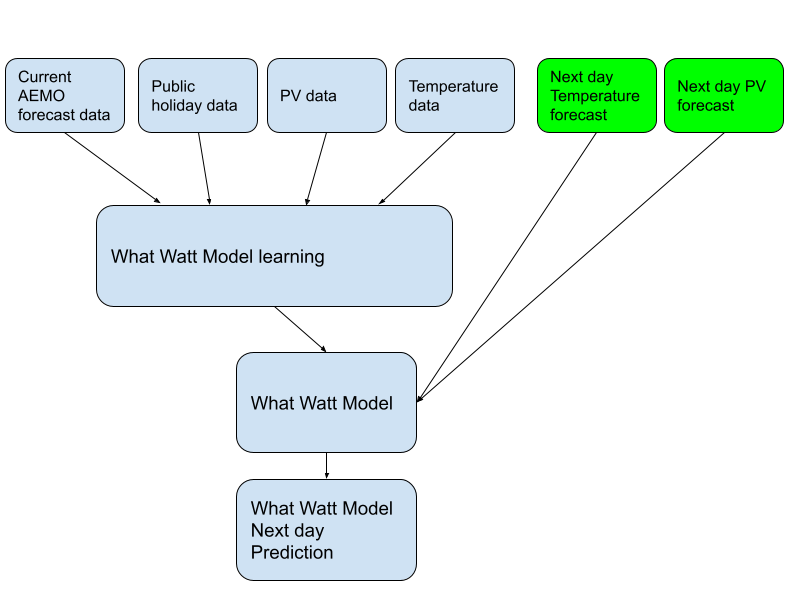
\includegraphics[width=140mm]{system.png}
\caption{Context diagram of the proposed energy forecasting model}\label{system}
\end{figure}

The historical data is provided to train the model. The forecast
temperature, and PV data, and the forecast demand data would be added
for the model to make a prediction.

\hypertarget{literature-review}{%
\chapter{Literature Review}\label{literature-review}}

In 1879 it was realised that the construction of the Garden Palace in
the domain in Sydney was unlikely to be completed in time, as such the
Goverment at the time decided to work at night. Arc lighting was chosen
to illuminate the site \cite{brady_1996_a}. The demand forecasting
process was slow, as was the electricity supply it required several
electrical generators to be procured and shipped from
England\cite{jobson_2004_power}.

As noted by Brady significant events in australian history have been as
a result of electricty demand, these include metallurgical industry in
1914, The Snowy Hydro scheme beginning in 1949 \cite{brady_1996_a} these
have had significant impact in shaping Australia.

Bently describes how the oil crisis in 1971 led to the need for better
and more accurate energy forecasting \cite{bentley_2002_oil}. It was
also around this time that it was recognised that the speed of
forecasting was important to manage not just the long term demand, but
also the change in demand across the duration of a day.

In 1997 NSW opted to privatise the energy
industry\cite{smith_1997_electricity} and systems needed to be put into
place to ensure that the market was able to match supply and demand of
electricity. Electricity requires the demand to equal supply for the
electrical grid to remain operational, if there is a increase or
decrease in the supply compared to the demand, then the frequency of the
electricity supply moves away from the Australian standard of 50hz, and
if moving to far away may result in a catastrophic failure of the
electrical grid.

Up until 2007 the majority of electrical supply was provided by the main
market players, with coal and the commercial green energy suppliers
providing to the market. In 2007 there was a move towards rooftop solar,
which is a system whereby individual households were able to generate
electricity that would be supplied into the grid. The systems in place
to match the electrical supply with the electrical demand, did not
include the rooftop solar. This is due to the fact that the rooftop
solar provides electricity to the house it is on, and that house's
energy demand is not included into the forecast that is available to be
sold to the electrical grid.

The rooftop solar has continued to grow, in 2007 it was 0.2\% of the
household roofs, whereas in 2020 it had moved to 20\% of houses having
rooftop solar, and using photovoltaic cells to generate local
electricity\cite{aemo_2020_projections}.

As the uptake and increase of rooftop solar has increased, this has
resulted in greater difficulty in modeling forecast
demand\cite{parkinson_2019_rooftop}. The fact that an increasing number
of houses are providing their own electricity for periods of the day
means that the variance in electricity forecast reliability decreases.
Currently the electricity used by domestic households for heating and
cooling is 32\%-33\% of total domestic energy use and is expected to
remain steady at around that number\cite{rgevorsatz_2015_heating}.This
heating and cooling is driven by the air temperature, and is the reason
why temperature is a key focus area in predicting energy demand.

The modeling methods of energy demand has changed in line with the
changes in energy usage. When the Snowy Hydro first came in the majority
of the electricity demand was from industry, and highly predictable,
there was less need for highly sophisticated modeling, however as the
domestic appliances, heating and cooking all moved to be driven by
electricity the need to model in a more granular way became essential.
In the 1970s the modeling was based on simple time linear
equations\cite{pawar_2020_predicting}\cite{griffin_1993_methodological}.
Since then modeling has improved to move towards more robust linear
models, and then through to time series modeling, and then more recently
neural networks\cite{marcjasz_2008_neural}. Modeling has included linear
neural networks and LSTM neural networks and MLPRegressor networks.

The focus of the modeling has been 2 fold, one to increase the accuracy
of the forecast, but just as importantly to decrease the maximum errors,
when the forecast model provides a result that turns out to be vastly
different to the actual demand, then there is significant strain on the
electrical grid. When there is a large difference between the forecast
and the actual demand it is necessary for the electrical suppliers to be
able to respond rapidly to ensure the stability of the frequency in the
network. In terms of speed to respond, Coal takes the longest, pumped
hydro and hydro the next, solar and wind (assuming conditions are
favourable), faster still and the quickest is the new grid connected
battery farms that can respond in microseconds.

\hypertarget{material-and-methods}{%
\chapter{Material and Methods}\label{material-and-methods}}

\hypertarget{software}{%
\section{Software}\label{software}}

All models in this report (except for Time Series) have been built using
Python via Google Colab, Table \ref{tab:python} shows the libraries and
machine lerning models used.

\begin{table}[H]
\centering
\begin{tabular}{p{0.3\linewidth} | p{0.6\linewidth}} 
\hline\hline
\textbf{Library}      & \textbf{Description}                                                                                                                         \\ 
\hline\hline
pandas                & Open source data analysis and manipulation tool.                                                                                             \\
numpy                 & Fundamental package for scientific computing with Python.                                                                                    \\
seaborn               & Statistical data visualization.                                                                                                              \\
matplotlib            & Creating static, animated, and interactive visualizations.                                                                                   \\
plotnine              & Grammar of graphic, based on ggplot2                                                                                                         \\
sklearn               & Simple and efficient tools for predictive data analysis.                                                                                     \\
plotly                & interactive, publication-quality graphs.                                                                                                     \\
XGBoost               & Efficient and portable optimized distributed gradient boosting.                                                                              \\
statsmodels           & Estimation of many different statistical models.                                                                                             \\
scipy                 & User-friendly and efficient numerical routine.                                                                                               \\
keras                 & Deep learning framework.                                                                                                                     \\
MLPRegressor~         & Multi-layer Perceptron regressor, optimises the squared-loss using LBFGS or stochastic gradient descent.                                     \\

LSTM       & Long Short-Term Memory, a model capbale to learn based on order dependance in sequence.                            \\

\hline\hline
\end{tabular}
\caption{python libraries and models used in the project}
\label{tab:python}
\end{table}

The Time Series model was built using R \&
RStudio\cite{rcoreteam_2017_r}, with the libraries in Table
\ref{tab:Rmodel}. All scripts used to produce the models and results in
this report are available on GitHub.

\begin{table}[H]
\centering
\begin{tabular}{p{0.3\linewidth} | p{0.6\linewidth}} 
\hline\hline
\textbf{Library}      & \textbf{Description}                                                                                                                         \\ 
\hline\hline
data.table & A data format used in R.                         \\
dplyr      & Used for data manipulation and transformations.  \\
forecast   & Methods  Tools to conduct time series analysis.  \\
lubridate  & Tools for transforming data/time variables.      \\
psych      & Produces summary statistics of data.            \\

\hline\hline
\end{tabular}
\caption{R libraries used in the project}
\label{tab:Rmodel}
\end{table}

For EDA, Power BI was used to produce visuals that explain trends and
relationships between variables. Data visualisations produced by Power
BI are included throughout this report, and the PowerBI code used is
available in GitHub.

This report was produced using Rmarkdown and MS SQL Server was used to
process the PV data to use for the model\cite{yihuixie_2018_r}.

\hypertarget{description-of-the-data}{%
\section{Description of the Data}\label{description-of-the-data}}

The data provided consisted of 3 csv files, all the files are
rectangular. The file forecastdemand\_nsw.csv is 739.63 MB in size and
consists of 6 columns and 10,906,019 rows. The type of data is shown in
Table \ref{tab:forecast_demand}. This data has been generated by the
AEMO\cite{aemo_electicity}.

\begin{table}[H]
\centering
\begin{tabular}{lll} 
\hline\hline
\textbf{Column Name} & \textbf{Python Data Type} & \textbf{Variable type}  \\ 
\hline\hline
PREDISPATCHSEQNO     & Int64                     & Discrete                \\
REGIONID             & object                    & Categorical 1 Value     \\
PERIODID             & int64                     & Categorical             \\
FORECASTDEMAND       & float64                   & Continuous              \\
LASTCHANGED          & object                    & Discrete                \\
DATETIME             & object                    & Discrete                \\
\hline\hline
\end{tabular}
\caption{Forecast demand data properties}
\label{tab:forecast_demand}
\end{table}

The file totaldemand\_nsw.csv is 5.80 MB in size and consists of 3
columns. The type of data is shown in Table \ref{tab:total_demand}

\begin{table}[H]
\centering
\begin{tabular}{lll} 
\hline\hline
\textbf{Column Name} & \textbf{Python Data Type} & \textbf{Variable type}  \\ 
\hline\hline
Column Name & Python Data Type & Variable type        \\
DATETIME    & object           & Discrete             \\
TOTALDEMAND & float64          & Continuous           \\
REGIONID    & object           & Categorical 1 Value \\
\hline\hline
\end{tabular}
\caption{Total demand data properties}
\label{tab:total_demand}
\end{table}

The file temperature\_nsw.csv is 6.877450MB in size and consists of 3
columns.The type of data is shown in Table \ref{tab:temperature}

\begin{table}[H]
\centering
\begin{tabular}{lll} 
\hline\hline
\textbf{Column Name} & \textbf{Python Data Type} & \textbf{Variable type}  \\ 
\hline\hline
LOCATION             & object                    & Categorical 1 Value     \\
DATETIME             & object                    & Continuous              \\
TEMPERATURE          & object                    & Continuous             \\
\hline\hline
\end{tabular}
\caption{Temperature data properties}
\label{tab:temperature}
\end{table}

The additional data we sourced was PV data, and public holiday data.
Both files are rectangular, the file ``NSW Public Holidays.csv'' is
8713B in size and consists of 5 columns and 135 entries, this was
sourced from the Digital Transformation Agency \cite{_australian} and
then had additional lines added taken from online calendars. The type of
data is shown in Table \ref{tab:public}

\begin{table}[H]
\centering
\begin{tabular}{lll} 
\hline\hline
\textbf{Column Name} & \textbf{Python Data Type} & \textbf{Variable type}  \\ 
\hline\hline
Year\_Date  & Datetime         & Discrete    \\
Day         & object           & Categorical    \\
Holiday     & object           & Categorical    \\
Type        & object           & Categorical    \\
Other       & object           & Categorical    \\
\hline\hline
\end{tabular}
\caption{Public Holiday data properties}
\label{tab:public}
\end{table}

We downloaded PV performance data for different NSW regions and PV
installation size for NSW and processed those files by using MS
SQL\cite{_2021_australian}. The type of data for the sites is shown in
Table \ref{tab:pvSite} and for installations in Table
\ref{tab:pvInstall}

\begin{table}[H]
\centering
\begin{tabular}{lll} 
\hline\hline
\textbf{Column Name} & \textbf{MS SQL Data Type} & \textbf{Variable type}  \\ 
\hline\hline
Location                            & Varchar(200)        & Categorical 1 value    \\
Timestamp                           & Datetime            & Discrete      \\
Irradiance(W/m2)                    & Decimal(28,3)       & Continous    \\
System temperature (C)              & Decimal(28,3)       & Continous      \\
Nearest BOM station temperatur (C)  & Decimal(28,3)       & Continous    \\
PV Yield (kWh)                      & iDecimal(28,3)      & Continous      \\
\hline\hline
\end{tabular}
\caption{NSW Regions Photo Voltaic data properties}
\label{tab:pvSite}
\end{table}

\begin{table}[H]
\centering
\begin{tabular}{lll} 
\hline\hline
\textbf{Column Name} & \textbf{MS SQL Data Type} & \textbf{Variable type}  \\ 
\hline\hline
Month                            & Varchar(50)        & Categorical 1 value    \\
lt2.5kW                           &int          & Continous      \\
2.5–4.5                    &int          & Continous    \\
4.5–6.5              &int       & Continous      \\
6.5–9.5  &int       & Continous    \\
9.5–14                      &int      & Continous      \\
14–25                    &int          & Continous    \\
25–50              &int       & Continous      \\
50–100  &int       & Continous    \\
100kW–5MW                      &int      & Continous      \\
5MW–30MW              &int       & Continous      \\
30+ MW  &int       & Continous    \\
Total Size (KW)                      &int      & Continous      \\
\hline\hline
\end{tabular}
\caption{NSW Regions Photo Voltaic data properties}
\label{tab:pvInstall}
\end{table}

The file PVGenerationNSWACT-30+MW-Excluded-2012\_032021.csv is 3.37MB in
size and consists of 162144 rows and consists of 2 columns.The type of
data is shown in Table \ref{tab:pv} The file was the final dataset
extracted from MS SQL.

\begin{table}[H]
\centering
\begin{tabular}{lll} 
\hline\hline
\textbf{Column Name} & \textbf{Python Data Type} & \textbf{Variable type}  \\ 
\hline\hline
DateTime         & object           & Discrete    \\
PVGeneration(MW) & int64            & Continous      \\

\hline\hline
\end{tabular}
\caption{Photo Voltaic generation data properties}
\label{tab:pv}
\end{table}

\hypertarget{pre-processing-steps}{%
\section{Pre-processing Steps}\label{pre-processing-steps}}

The following three data sets containing historical data from 01 January
2010 were shared through a GitHub repository. These files where the ones
provided as initial input to the electicial modeling problem.\\

\begin{itemize}
\item Total electricity demand
\item Forecast demand
\item Air Temperature
\end{itemize}

We also used the following two external data sets for this project.

\begin{itemize}
\item NSW public holiday data
\item Rooftop Solar PV data
\end{itemize}

To work in Python the GitHub repository was cloned and a data folder was
created. There were two files for the forecast demand which merged into
one file. All three data files were unzipped and stored as .csv in the
data folder.

\hypertarget{total-electricity-demand-data}{%
\subsection{Total electricity demand
data}\label{total-electricity-demand-data}}

The Total electricity demand in megawatt is half-hourly increments
demand for New South Wales. This data is sourced from the Market
Management System database, which is published by the market operator
from the National Electricity Market (NEM) system.

\hypertarget{importing-total-electricity-demand-data}{%
\subsection{Importing total electricity demand
data}\label{importing-total-electricity-demand-data}}

The data from the totaldemand\_nsw.csv was stored into a dataframe.

\hypertarget{forecast-demand-data}{%
\subsection{Forecast demand data}\label{forecast-demand-data}}

The Forecast demand data is the half-hourly increments of electricity
demand in megawatt for New South Wales. This data is also sourced from
the Market Management System database.

\hypertarget{importing-forecast-demand-data}{%
\subsection{Importing forecast demand
data}\label{importing-forecast-demand-data}}

The data from the forecastdemand\_nsw.csv was stored into a dataframe.

\hypertarget{air-temperature-data}{%
\subsection{Air temperature data}\label{air-temperature-data}}

The air temperature data for New South Wales was measured from the
Bankstown Airport weather station. This data is sourced from the
Australian Data Archive for Meteorology.

\hypertarget{importing-air-temperature-data}{%
\subsection{Importing air temperature
data}\label{importing-air-temperature-data}}

The data from the temperature\_nsw.csv was stored into a dataframe
df\_temp.

\hypertarget{nsw-public-holiday-data}{%
\subsection{NSW Public Holiday Data}\label{nsw-public-holiday-data}}

The NSW public holiday data was taken from Digital Transformation Agency
for 2014 onwards, and then manually updated with the 2010 through to
2014 based on searching old calendars\cite{_australian}.

\hypertarget{importing-public-holiday-data}{%
\subsection{Importing public holiday
data}\label{importing-public-holiday-data}}

The public holiday data was loaded into a DataFrame df\_publicholidays
from NSW Public Holidays.csv.

\hypertarget{rooftop-solar-pv-data}{%
\subsection{Rooftop Solar PV Data}\label{rooftop-solar-pv-data}}

Following two different data sources related to solar PV were downloaded
from (Australian PV Institute (APVI) Solar Map) for January 2010 to
March 2021 period \cite{_2021_australian}.

\begin{itemize}
\item Solar PV performance data for several regions of NSW
\begin {itemize}
\item Canterbury (NSW)
\item Sutherland (NSW)
\item St Ives (NSW)
\item Newtown (NSW)
\end{itemize}
\item Cumulative PV installation size data for NSW and ACT regions 
\end{itemize}

\hypertarget{importing-rooftop-solar-pv-data}{%
\subsection{Importing Rooftop Solar PV
Data}\label{importing-rooftop-solar-pv-data}}

We used MS SQL Server database to store and process the data to prepare
the final PV Data set to load into Python DataFrame for the model.

\begin{itemize}
\item Both solar PV data sets were loaded in MS SQL Server database by using SQL Server Import and Export Wizard.
\item As the size of a single PV unit for different locations are different (see Table \ref{tab:pv_size}), we normalised the PV Yield (kWh) value for a PV unit size of 5kWp for all locations.
\end{itemize}

\begin{table}[H]
\centering
\begin{tabular}{ll} 
\hline\hline
\textbf{Region}  & \textbf{Single PV system size (kWp)}  \\ 
\hline\hline
Canterbury (NSW) & 3.06                                  \\
Sutherland (NSW) & 5.04                                  \\
St Ives (NSW)    & 5.1                                   \\
Newtown (NSW)    & 5.1                                   \\
\hline\hline
\end{tabular}
\caption{Photo Voltaic generation region and single system size}
\label{tab:pv_size}
\end{table}

\begin{itemize}
\item Prepared a dataset by using only Canterbury PV performance data as this region has been considered as a representative of NSW solar PV data (see Section \ref{pvSiteAssume} for detailed explanation).  
\item The missing dates of Canterbury were filled by using either Sutherland or St Ives or Newtown data.
\item Canterbury solar PV performance data is for every hour interval. We converted the data to make a 30 minutes interval of solar power production byhalving the hourly data. 
\item PV installation of size 30+MW excluded from the dataset during calculating the total cumulative size of PV installation for NSW for every month\cite{brinsmead_2014_energy} we normalised the PV Yield (kWh) value for a PV unit size of 5kWp for all locations (see Section \ref{30MW} for details).
\item Final dataset was exported as a csv file.
\item The final rooftop solar PV generation data was loaded into a DataFrame.
\item We prepared a dataset for every 30 minutes interva by using solar power generation for NSW by multiplying Canterbury data with the total capacity of NSW PV for that date and time. The PV capacity data was based on monthly totals and we assumed a linear rollout of the PV across that month (this had small impact on the total numbers but was a reliable method).
\end{itemize}

\hypertarget{data-cleaning}{%
\section{Data Cleaning}\label{data-cleaning}}

Data cleaning is an essential part of every machine learning project to
get better and accurate models. The following summarizes the data
cleaning steps that we undertook.

\hypertarget{cleaning-total-electricity-demand-data}{%
\subsection{Cleaning total electricity demand
data}\label{cleaning-total-electricity-demand-data}}

\begin{itemize}
\item The total demand data was time series data with values of total demand for every 30 minutes, this was treated as the ground truth and the sampling period that the rest of the data would be aligned to. 
\item The DATETIME column was imported as an Object which was converted to python Datetime. 
\item we set the DataFrame index by using DATETIME
\end{itemize}

\hypertarget{cleaning-forecast-demand-data}{%
\subsection{Cleaning forecast demand
data}\label{cleaning-forecast-demand-data}}

\begin{itemize}
\item The DATETIME column of forecast DataFrame was imported as an Object which was converted to python Datetime. 
\item we set the DataFrame index by using DATETIME
\item The Forecast Demand data had one or more values for each of the 30 minutes time periods. As the later values represented the most recent output from the NEMS forecast demand, the most recent forecast demand was considered ,as this was the output from the model which had the most up-to-date input data.
\end{itemize}

\hypertarget{cleaning-air-temperature-data}{%
\subsection{Cleaning air temperature
data}\label{cleaning-air-temperature-data}}

\begin{itemize}
\item The DATETIME column of temperature DataFrame was imported as an Object which was converted to python Datetime. 
\item We set the DataFrame index by using the DATETIME column.
\item The temperature data was a time series that was more asynchronous and could contain multiple values for the 30 minute target time. This data was always relatively close to each other so an arithmetic mean was used to create the single value for the 30 minute period.
\end{itemize}

\hypertarget{cleaning-public-holiday-data}{%
\subsection{Cleaning public holiday
data}\label{cleaning-public-holiday-data}}

\begin{itemize}
\item Renamed the column Year Date to DATETIME
\item Excluded pre 2012 data from the DataFrame
\item Added a flag column PUBLICHOLIDAYS
\item Set the DataFrame index by using the DATETIME column.
\item Dropped unused columns Day, Holiday, Type and Other
\item Resampled the public holiday data for everyday
\item Updated  flag column PUBLICHOLIDAYS with 0 for non public holidays
\item Resampled the public holidays DataFrame for 30 minutes interval
\end{itemize}

\hypertarget{cleaning-solar-pv-data}{%
\subsection{Cleaning solar PV data}\label{cleaning-solar-pv-data}}

\begin{itemize}
\item The DateTime column of solar pv DataFrame was imported as an Object which was converted to python Datetime. 
\item Set the DataFrame index by using DateTime 
\item Renamed the column DateTime to DATETIME
\end{itemize}

\hypertarget{adding-features-to-forecast-demand-data}{%
\subsection{Adding features to forecast demand
data}\label{adding-features-to-forecast-demand-data}}

\begin{itemize}
\item Added hour, Minute, HourMinute, Month, Year, Day, DayName as extra columns
\item Added season based on Month from December to February as ‘Summer’, March to May as ‘Autumn’, June to August as ‘Winter’ and September to November as ‘Spring’
\end{itemize}

\hypertarget{adding-features-to-temperature-data}{%
\subsection{Adding features to Temperature
data}\label{adding-features-to-temperature-data}}

Added temperature classification which is grouped into 5 different
ranges.

\begin{itemize}
\item Less than or equal 10 degree C: very low
\item Between 10 and 20: low
\item Between 20 and 30: high
\item Between 30 and 35: very high
\item More than or equal to 35: extremely high
\end{itemize}

\hypertarget{merging-all-dataframes}{%
\subsection{Merging All DataFrames}\label{merging-all-dataframes}}

Created a dataframe df\_final by merging all five dataframes
(df\_forecast\_merge, df\_temp\_merge, df\_totaldemand,
df\_publicholidays\_merge, df\_pv)

One hot coding on columns which have categorical data, as we have
introduced categorical data into our datasets, we were required to apply
one-hot encoding techniques in order to use these features in our
models. One-hot encoding expands each possible value of a categorical
variable into multiple binary columns, so that these features can be
interpreted by the
models\cite{httpswwwfacebookcommachinelearningmastery_2017_why}. The
following categorical variables were transformed using one-hot encoding:

\begin{itemize}
\item Seasonal categorical data
\item 0 or 30 minute categorical data
\item Temperature categorical data
\end{itemize}

\hypertarget{assumptions}{%
\section{Assumptions}\label{assumptions}}

\begin{itemize}
\item The forecast demand data had one or more values for each of the 30 minutes time periods. As the later values represented the most recent output from the NEMS forecast demand, the most recent forecast demand was considered  as this was the output from the model which had the most up-to-date input data\cite{abcb_2015_climate}.
\item \label{pvSiteAssume}Assume the PV data at Canterbury was representative of the PV data across the highest demand area of the state (the Sydney / Newcastle / Wollongong areas). The figure \ref{assume} shows the comparison of PV performance for Canterbury and St Ives. Figure \ref{Cant} in the Appendix shows the comparioson with Sutherland\cite{abcb_2015_climate}.
\begin{figure}[H]
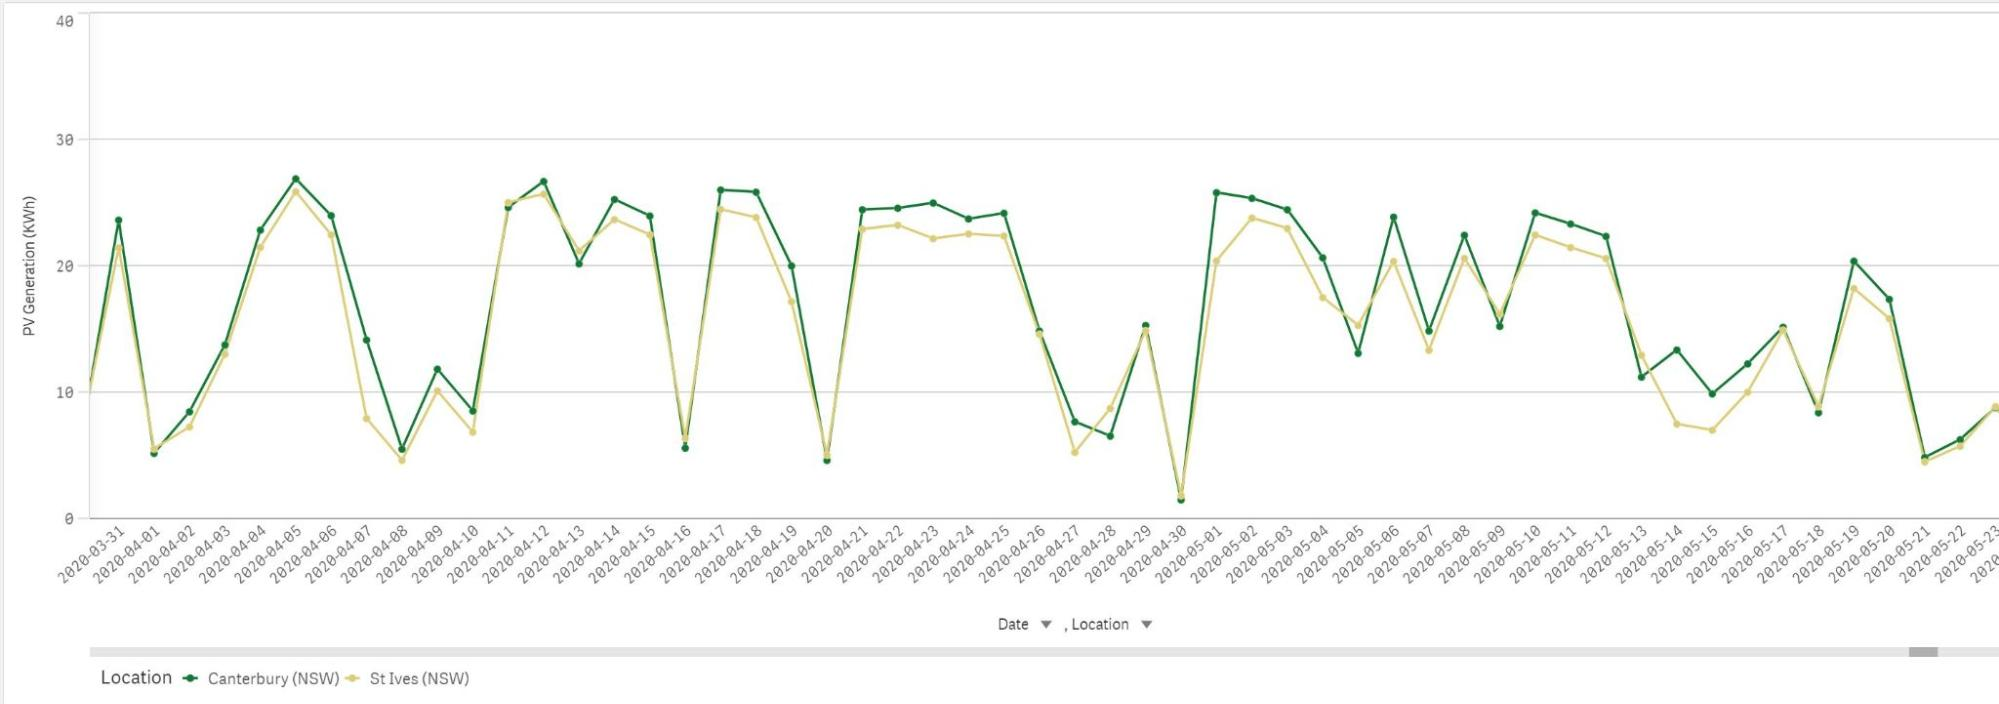
\includegraphics[width=140mm]{image25.jpg}
\caption{PV Performance comparison between Canterbury and St Ives generated by single 5Kwp system }
\label{assume}
\end{figure}
\item \label{30MW}We have assumed that the  30+MW size solar PV systems are part of the Energy Grid, and participate in the energy spot market. This means that their capacity is included in the total demand / forecast, and as such should be excluded from our PV data, which is to represent  supply that is not part of the spot market\cite{brinsmead_2014_energy}.
\item The temperature at Bankstown airport is indicative of the entire state. This assumption is based on the similarity of climate zones\cite{abcb_2015_climate} where the majority of the energy demand is from.
\item To minimise the possibility of multicollinearity, variables were removed from the training dataset based on their Variance Inflation Factor (VIF). Should a variable have a high VIF, then that variable would be removed as it significantly increases the variable of parameter estimates due to high correlation with other variables. The generally accepted rule in the industry is that a variable with a VIF greater than 10 should be removed, Table \ref{VIF} in the Appendix shows how the rule was applied to our variable selection criteria\cite{pvatcheva_2016_multicollinearity}.
\item We assumed that 500 was a good value for the outliers, due to the natural split in the data when viewed, this can be infered from Figure \ref{image16}.
\end{itemize}

\hypertarget{modelling-methods}{%
\section{Modelling Methods}\label{modelling-methods}}

Due to research such as Almalaq et al \cite{almalaq_2017_a} and Marcjasz
et al \cite{marcjasz_2008_neural} We decided to use several different
models to improve the RMSE comparatively against the AEMO data. The
first, simple model that we chose was an ARIMA time series model, this
was to help us get an understanding of the data, and what we might be
able to expect from future modeling. We then chose to use a MLP
Regressor model, and XGBoost model, and an LSTM model. The MLPRegressor
would act as a sliding window across the data, building up a good
representation of the data, the XGBoost uses a regulated Gradient
Descent approach that should assist with identifying outliers, and the
LSTM was chosen as it should provide the capability of understanding the
previous steps, similar to ARIMA as well as pick up on the features more
accurately similar to the MLPRegressor and XGBoost models.

\hypertarget{exploratory-data-analysis}{%
\chapter{Exploratory Data Analysis}\label{exploratory-data-analysis}}

The first step in our exploration of the data was to visualise the
target output, in this case total demand. The figure \ref{image12} shows
the scatter plot of total demand and the figure \ref{image32} shows the
forecast demand and the figure \ref{image63} shows the scatter plot of
the difference between total deamnd and forecast demand averaged across
a day. As can be seen, the data has a slow trend downwards over the year
with weekly cycles. The forecast demand had a high degree of
uncertainty. The years 2010-2012 had very high variance, and as a result
we dropped these from the modeling early.

\begin{figure}[H]
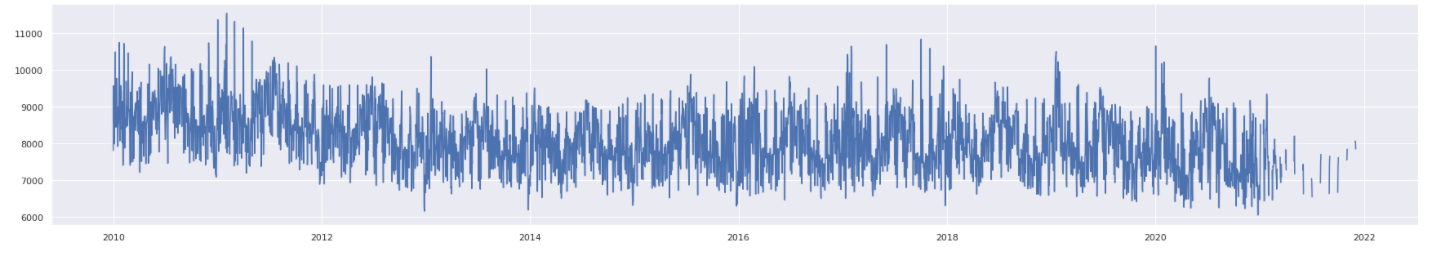
\includegraphics[width=140mm]{image12.png}
\caption{Total demand by datetime}
\label{image12}
\end{figure}

\begin{figure}[H]
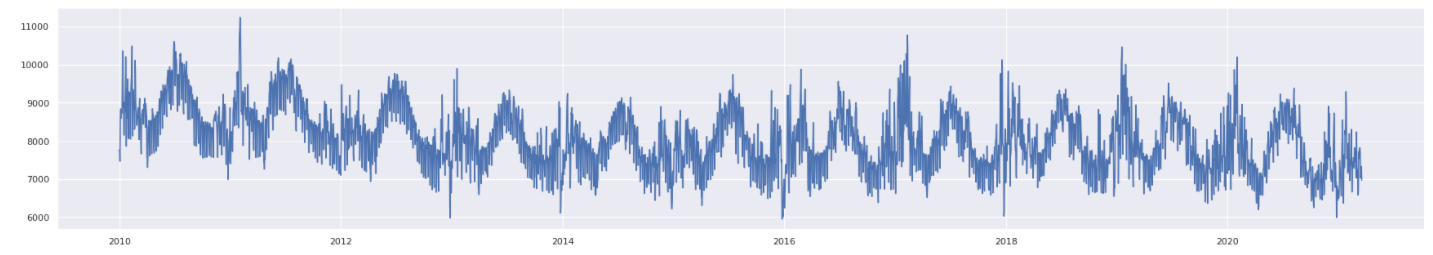
\includegraphics[width=140mm]{image32.png}
\caption{Total forecast by datetime}
\label{image32}
\end{figure}

\begin{figure}[H]
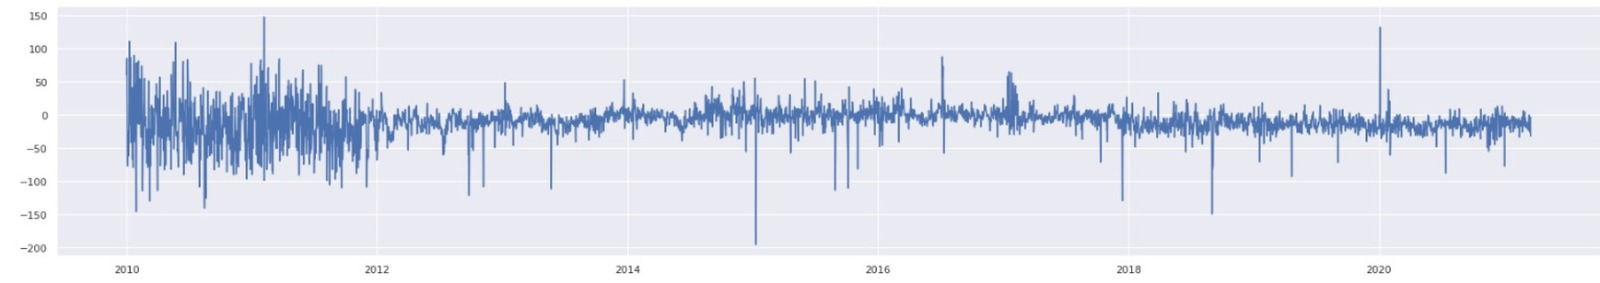
\includegraphics[width=140mm]{image63.jpeg}
\caption{Absolute difference between total demand and total forecast averaged across a day for 2010 to 2021}
\label{image63}
\end{figure}

In an effort to understand how the demand changed over the years we
graphed the probability density against the energy consumption, this
would enable us to see the similarity in the graphs as well as to see
how the peak value changed Figure \ref{image17} shows this information.
It was observed that the unimodal distribution for each year resulted in
a lower energy consumption each year. This shift is most likely be
caused by the increasing installation of rooftop solar panels and
specially in the 2020 the cause is the Covid-19 shutdown. With rooftop
solar not included in the total demand numbers this could be explained
by the addition of rooftop solar.

\begin{figure}[H]
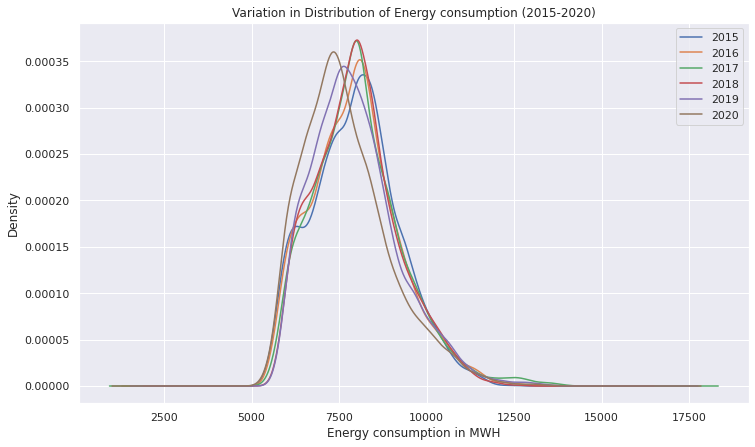
\includegraphics[width=140mm]{image17.png}
\caption{Difference between total demand and forecast vs Temperature for every year from 2015 to 2020}
\label{image17}
\end{figure}

As we were investigation the impact of PV energy in the model, it was
important to understand how the impact would be seen across the seasons.
During summer PV data should show a greater impact than in the winter.
To investigate this,we graphed the distribution for summer versus winter
as shown in figure \ref{image9}, the summer data was bimodal, compared
to the winter which was unimodal. Whilst the spread of the data was
similar between winter and summer the variation year on year increased,
with 2017-2019 are bimodal in summer, which is an indication of the
rooftop solar rolllout. The 2020 was moving more to the unimodal type
again, this could either be due to the large percentage of rooftop solar
impacting the data, or due to covid social impact changing how people
responded.

\begin{figure}[H]
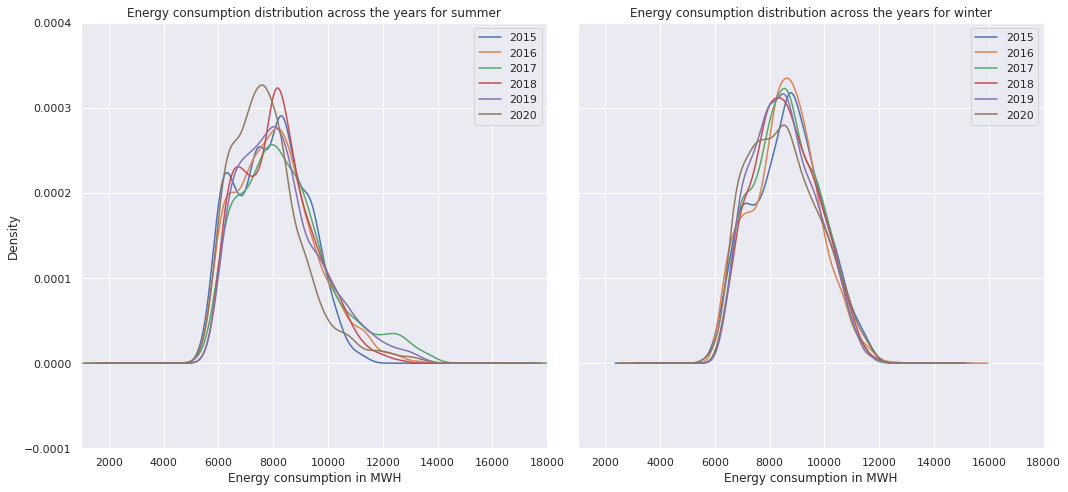
\includegraphics[width=140mm]{image9.png}
\caption{ Variation for summer and winter of total demand for the years 2015 to 2020}
\label{image9}
\end{figure}

In household and large corporations Ürge-Vorsatz et al show that the use
of electricity is often linked to either heating or cooling
\cite{rgevorsatz_2015_heating}. To see if this was an impact to our
model we did a scatter graph of total demand versus temperature. Figure
\ref{image25} shows that the total demand is lowest around 18-19 degrees
and increases the further you move away from that temperature. The data
shows that this is consistent across all the years from 2015 - 2020.

\begin{figure}[H]
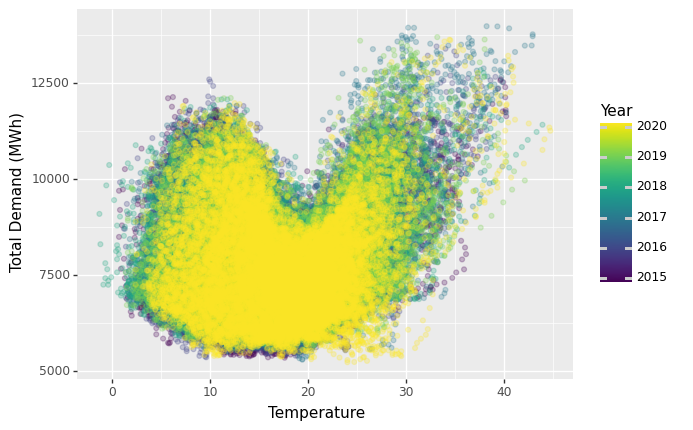
\includegraphics[width=140mm]{image25.png}
\caption{Difference between total demand and Forecast vs Temperature for every year from 2015 to 2020}
\label{image25}
\end{figure}

When looking at the overall scatter shown in Figure \ref{image12} it
could be seen that the data followed weekly cycles. To see if this was a
result in similarities between daily information or other influences, we
created a box plot of demand versus week day. Figure \ref{weekly} shows
that the week days are very similar and the weeknds separate again.
Mondays did have some similarities with weekend's this is likely due to
the fact that public holidays are often on a monday, and the demand on
those days is more similar to the weekend. As a result of this data we
chose to use weekday and public holiday data as features to include in
the modeling (this was then verified by the VIF we performed).

\begin{figure}[H]
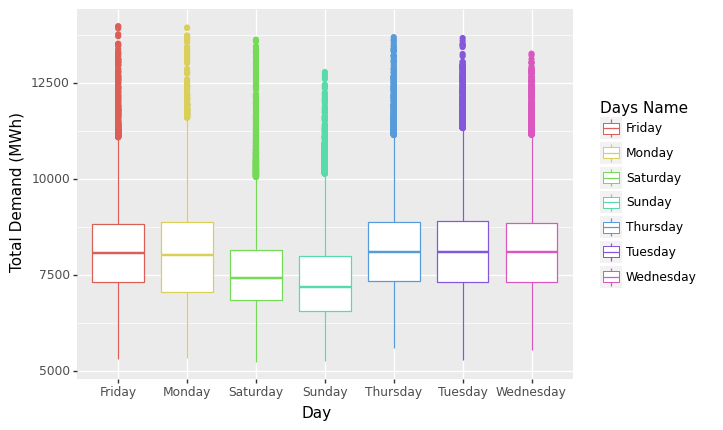
\includegraphics[width=140mm]{Electricity Total Demand distribution on week days for 2015 to 2020.png}
\caption{Electricity Total Demand distribution on week days for 2015 to 2020}
\label{weekly}
\end{figure}

Our focus was in identifying how we could improve the accuracy of
outlier days, as well as the accuracy of the overall model. For this we
needed to have a good understanding of where the outliers are. Figure
\ref{demandvtempbox1} is a box plot that shows the different quartiles
for each year form 2015 through to 2020.

\begin{figure}[H]
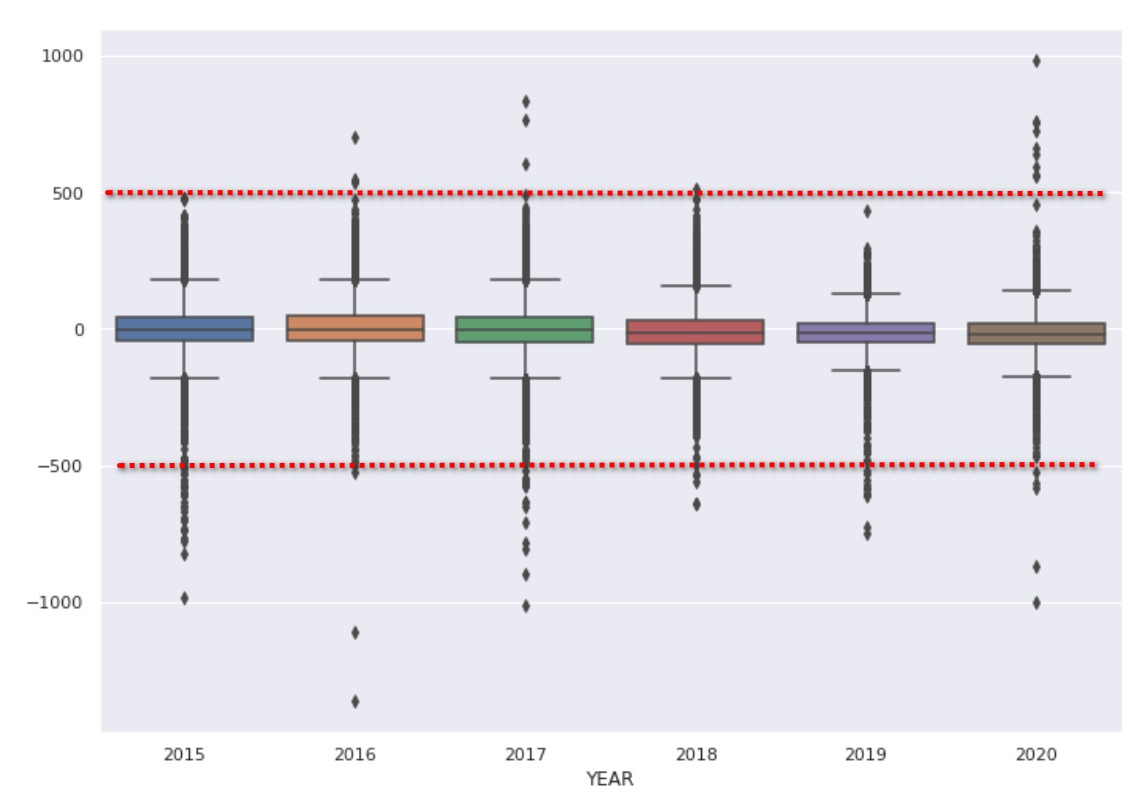
\includegraphics[width=140mm]{image200.jpg}
\caption{Distribution of the difference between Total demand and Forecast for every year from 2015 to 2020}
\label{demandvtempbox1}
\end{figure}

The output from the rooftop solars has been increasing over the last 10
years, whislt there has been a slow decline in the total demand, Figure
\ref{rtsolar} indicates that the increase in PV output is increasing it
does not account for the total decrease in total demand. Figure
\ref{RFSolar} in the Appendix visualises the growth of rooftop solar

\begin{figure}[H]
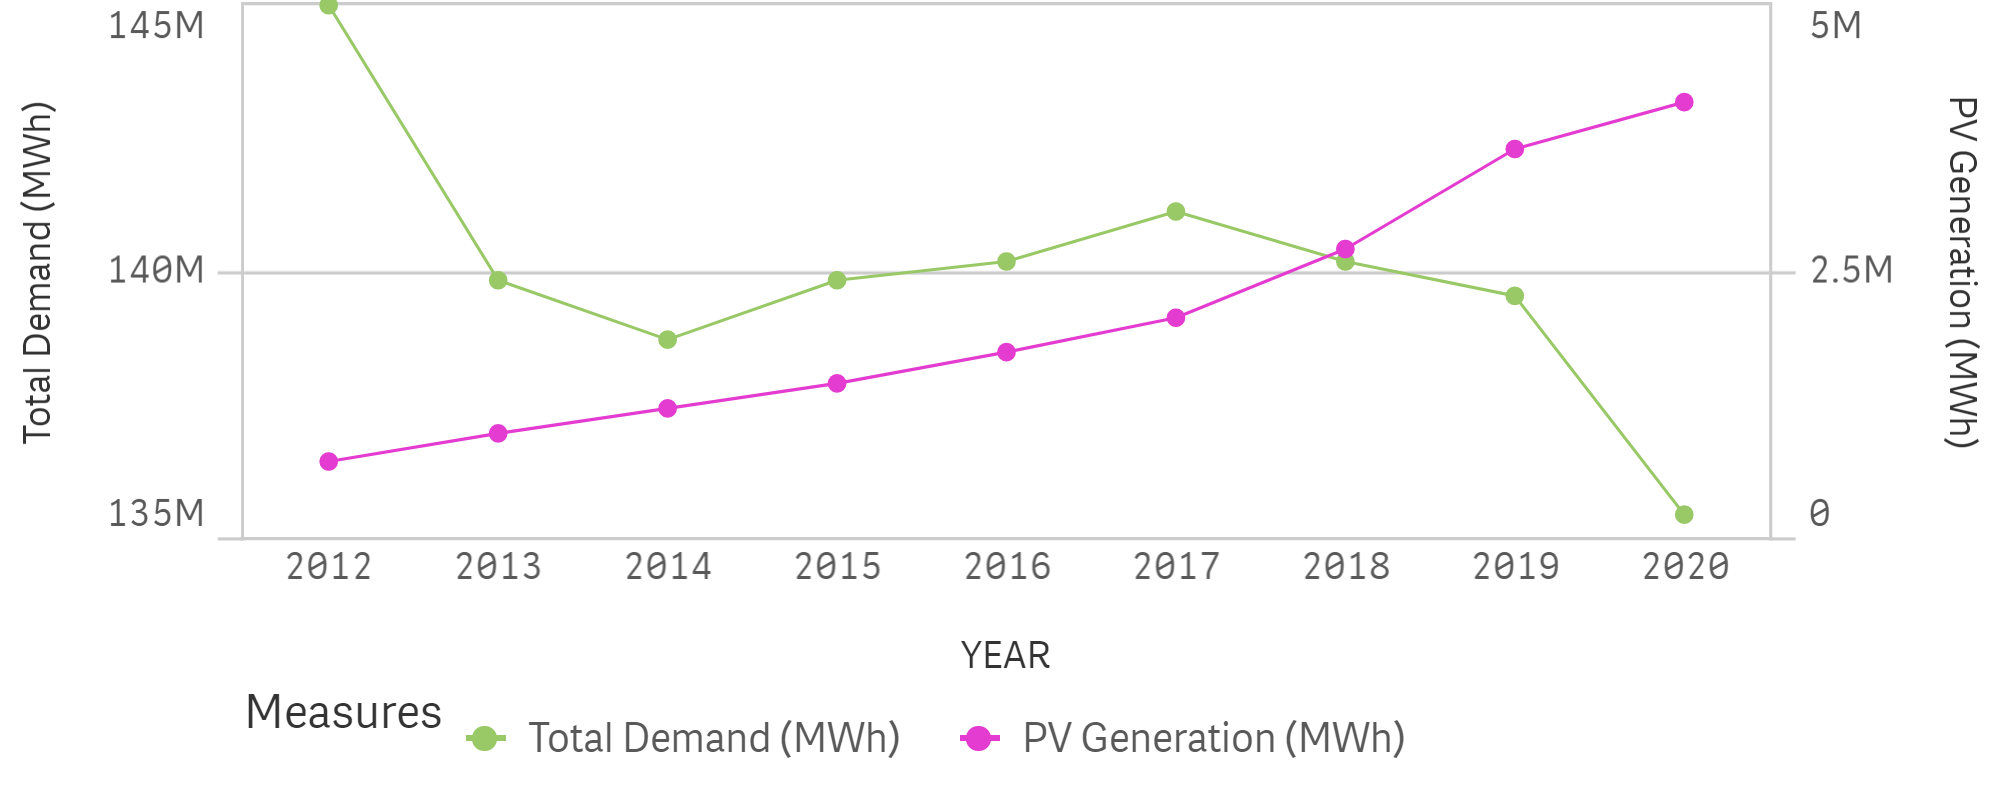
\includegraphics[width=140mm]{image3.png}
\caption{PV Generation vs Total Demand for 2012 to 2020}
\label{rtsolar}
\end{figure}

\hypertarget{analysis-and-results}{%
\chapter{Analysis and Results}\label{analysis-and-results}}

\hypertarget{arima---baseline-model}{%
\section{ARIMA - Baseline Model}\label{arima---baseline-model}}

Time series models are often used to predict future events when given
data that is provided in regular \& discrete time
intervals\cite{statistics_australian}. It is an especially useful
modelling tool when the data has a clear trend and/or seasonality
components, as these predictable features can be isolated via the
Box-Jenkins method, and an AutoRegressive Integrated Moving Average
model (ARIMA) can be applied. Time series models are commonly used in
stock price predictions, logistics management, sales forecasts and IoT
devices.

As the data for total demand was provided in regular 30-minute
intervals, and since there is a clear seasonality trend in the data, it
was decided that a time series model would be appropriate to use when
predicting future total demand.

The ARIMA model was trained on the first 80\% of the data (which
contains data from 1/1/12 to 16/5/19), and then tested the remaining
20\% of the data. Using the ``auto.arima'' function in R to find the
combination of p, d \& q that minimises the AIC. An ARIMA(4,1,2) model
was suggested to have the optimal set of parameters for the ARIMA, as
shown in Figure \ref{image33} below \cite{hyndman_2018_87}.
Mathematically, this equation is written below as, where \(\hat{X_t}\)
represents total demand at time t, and \(\epsilon_t\) represents the
error term at time t:

\[
\hat{X_t} = 0.8243X_{t-1} + 0.8931X_{t-2} - 0.7242X_{t-3} - 0.0681X_{t-4} + \epsilon_t - 0.0446\epsilon_{t-1} - 0.9328\epsilon_{t-2}
\]

The performance of the ARIMA(4,1,2) model has RMSE of 82.48 for 2020
which is higher than RMSE of the AEMO's model which is 74.15 which
indicated that the ARIMA(4,1,2) model performed poorer than the AEMO's
model for overall predictions (see Figure \ref{image33} ).

\begin{figure}[H]
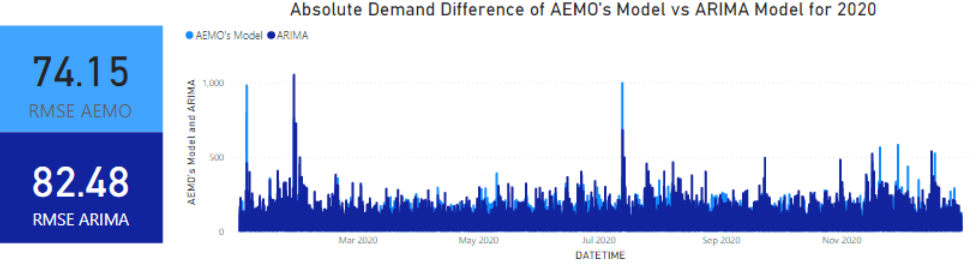
\includegraphics[width=140mm]{image33.png}
\caption{Absolute Demand Difference of AEMO's model versus ARIMA Model for 2020}
\label{image33}
\end{figure}

For outliers, the ARIMA(4,1,2) model has RMSE of 244.41 which is much
lower than RMSE of the AEMO's model which indicated that the
ARIMA(4,1,2) model performed much better for the outliers (see Figure
\ref{image7})

\begin{figure}[H]
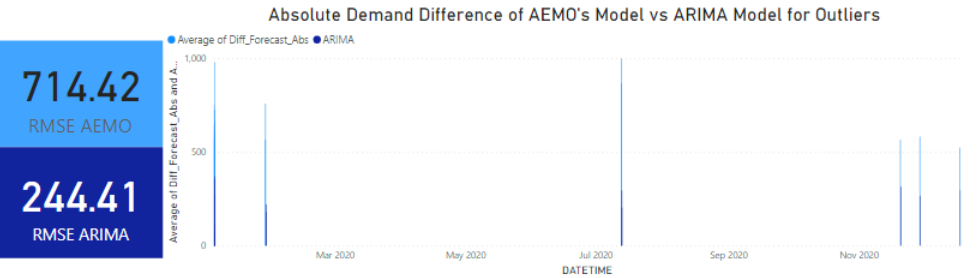
\includegraphics[width=140mm]{image7.png}
\caption{Absolute Demand Difference of AEMO's model versus ARIMA Model for outliers in 2020}
\label{image7}
\end{figure}

\hypertarget{neural-network-mlpregressor}{%
\section{Neural Network
MLPRegressor}\label{neural-network-mlpregressor}}

The MLPRegressor model acts as a sliding window across the data,
researchers such as Ozden et al.~have used MLPRegressor models to
forecast electricity demand, in their case it was to assist with
determining locations of where renewable power supplies should be
placed\cite{ozden_2018_prediction}.

We used 200 nodes in hidden layers as it offers the best output after we
tested using 50, 100, 200, 300, 400, 500 and 1000 nodes. We used the
relu activation function because it gives output between 0 and the
maximum value also Ozden et al.~used it in their research. We use ADAM
solver for weight optimisation as it offers the better output than SGD
solver. We use alpha L2 penalty (regularisation), termination parameter
as 0.001, the maximum number of iterations (max\_iter) as 5000, and the
tolerance for the optimisation as 0 as they offer better output than
others tested.

The overall performance of the MLPRegressor model was better than some
models in this paper (ARIMA, LSTM); however, XGBoost performed better
than MLPRegressor. It offers the optimal output with RMSE of 70.99
comparing to RMSE of 74.15 from the AEMO's model (see Figure
\ref{image333}). The reason is that because the MLPRegressor model
optimises the squared-loss using LBFGS or stochastic gradient descent.

\begin{figure}[H]
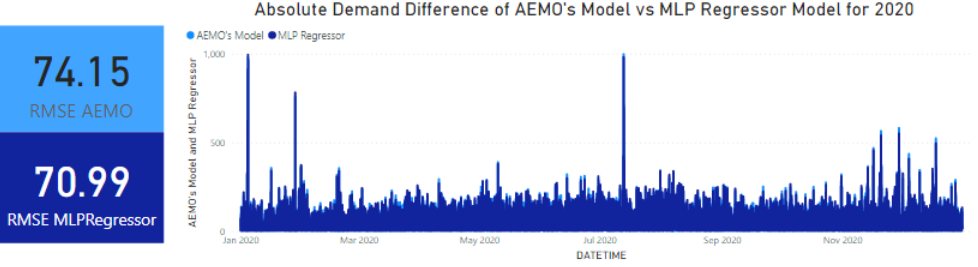
\includegraphics[width=140mm]{image4.png}
\caption{Absolute Demand Difference of AEMO's model versus MLPRegressor for 2020}
\label{image333}
\end{figure}

For the outliers, the MLPRegressor model outputs RMSE of 710.96 which is
lower compared to RMSE of 714.42 from the AEMO's model (see Figure
\ref{image13}). For the outliers days, MLPRegressor performs better than
XGBoost Regressor; however, not as good as ARIMA model which has
information about unusual events (for example, due to bushfires, COVID
lockdown) to be able to predict outliers correctly Figure \ref{XGTune}.

\begin{figure}[H]
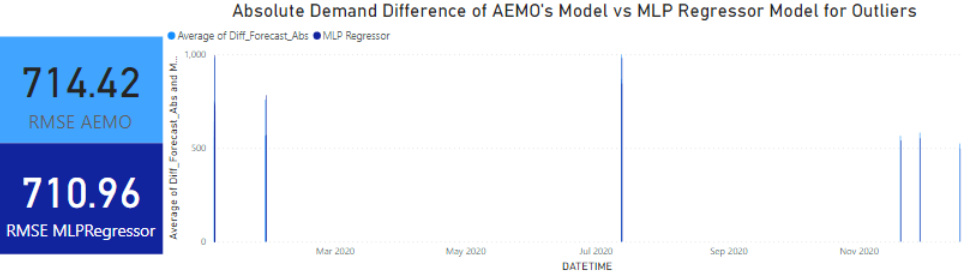
\includegraphics[width=140mm]{image13.png}
\caption{Absolute Demand Difference of AEMO's model versus MLP regressor Model for outliers in 2020}
\label{image13}
\end{figure}

\hypertarget{xgboost-regressor}{%
\section{XGBoost Regressor}\label{xgboost-regressor}}

The XGBoost Regressor model was trained on 2 recent years of data
between 2018 and 2019, including year 2021 data upto 17th March 2021 and
tested on one year of data in 2020. The model calls XGBRegressor library
in Python with 600 estimators, linear regression to train and test.
Using 600 estimators in this model offer the best output which is the
lowest RMSE as 67.35 comparing to using other number of estimators (see
Figure \ref{image1}).

\begin{figure}[H]
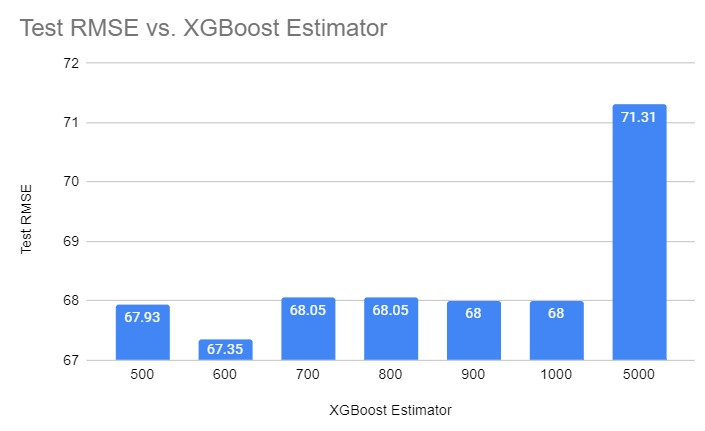
\includegraphics[width=140mm]{image1.jpg}
\caption{Test RMSE versus XGBoost Estimator}
\label{image1}
\end{figure}

The overall performance of the XGBoost Regressor model was greater than
other models in this paper (ARIMA, and LSTM). It offers the optimal
output with RMSE of 67.35 comparing to RMSE of 74.15 from the AEMO's
model (see Figure \ref{image2}). The reason is that XGBoost regressor
offers optimised implementation of gradient boosting which calculates
residual errors from the latest predictor and tried to fit the new
predictor to these residual errors. XGBoost includes a unique
split-finding algorithm to optimise trees, along with built-in
regularisation that reduces overfitting. It is scalable and very fast.
This model is also easy to tune with minimum parameters to tune and fast
to re-train.

\begin{figure}[H]
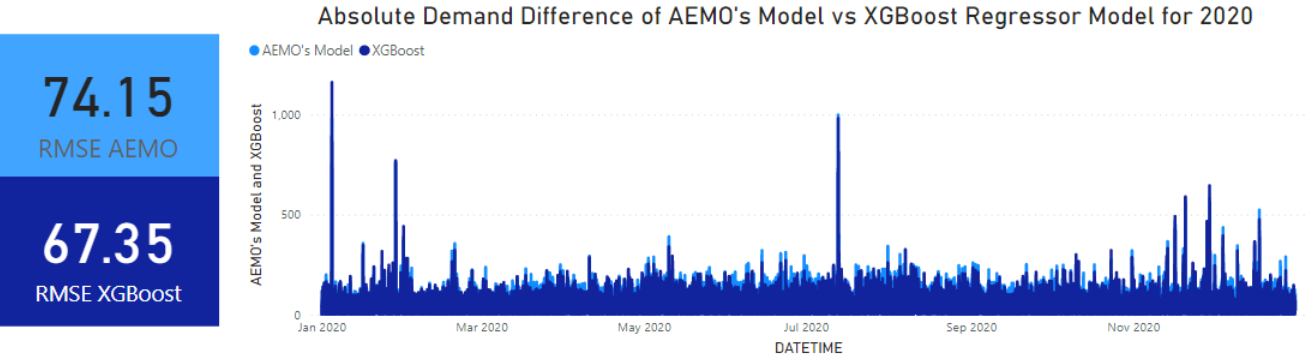
\includegraphics[width=140mm]{image2.png}
\caption{Absolute Demand Difference of AEMO's model versus XGBoost Regressor for 2020 }
\label{image2}
\end{figure}

For the outliers, the XGBoost Regressor model outputs RMSE of 741.26
which is higher compared to RMSE of 714.42 from the AEMO's model (see
Figure \ref{image24}). For the outliers day XGBoost Regressor performs
not as wel as ARIMA model as XGBoost Regressor does not have information
about unusual events (for example, due to bushfires, COVID lockdown) to
be able to predict outliers correctly Figure \ref{XGTune} in the
appendix shows this information.

\begin{figure}[H]
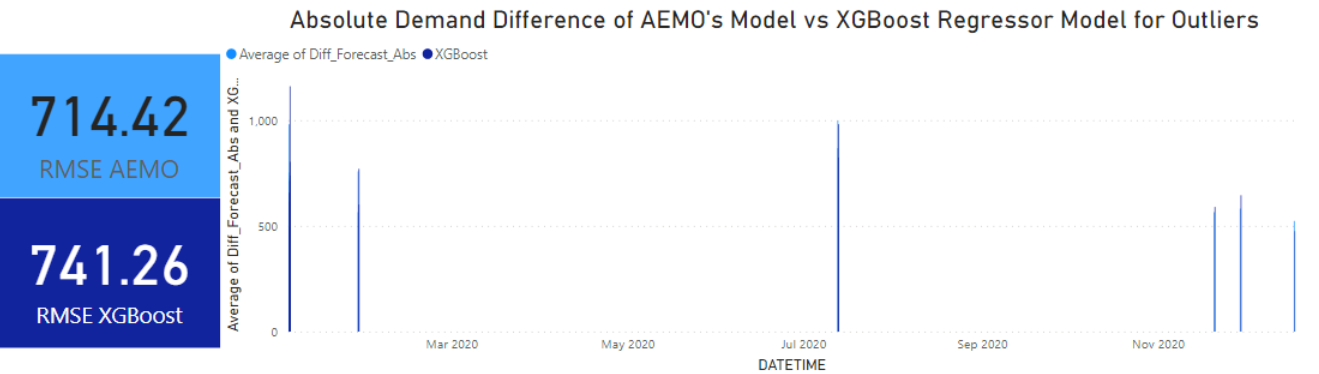
\includegraphics[width=140mm]{image24.png}
\caption{Absolute Demand Difference of AEMO's model versus XGB Regressor for Outliers in 2020}
\label{image24}
\end{figure}

XGboost has been used by researchers such as Almalaq et al to model
demand forecasts\cite{almalaq_2017_a}.

\hypertarget{lstm}{%
\section{LSTM}\label{lstm}}

The long short term memory models are often used to pick up non-linear
behaviour in time series data sets. The LSTM has the ability to build a
model that forgets information not relevant, and focuses on the long
term trends as well as the short term fluctuations. Researchers such as
Mesa Jiménez et al.~have used LSTM models to model demand, however they
also used exponentially moving averages to help capture the peaks in the
data. Due to the limitation in time, we used a naive approach to the
LSTM modeling\cite{mesajimnez_2020_modelling}.

We created a LSTM that consisted of 200 neurons (tested against 50, 100,
150 and 200), we also had a network that consisted of 4 layers, 3 LSTM
layers, the final with a 50\% dropout to avoid overfitting, and the
final being a fully connected dense layer to generate the predicted
total demand. The lag of the series consisted of only a single previous
value, and this naivete led to high RMSE value of 195.585, If additional
time, we would have built an LSTM that had a lag of 48 to be able to
have a full days history in the model. The additional layers should then
have been able to pick up more of the characteristics of the data. The
model was created by using 2 years worth of data, and with 2020 data as
the test data. As the LSTM requires normalised data, all the data
(including the one hot encoded data) was normalised to be between 0 and
1. The predicted total demand hours where then rescaled back so the data
could easily be compared. The naivety of the model and the lack of time
to improve its accuracy meant that we reverted to the MLPRegressor,
XGBoost models, and ARIMA models.

\hypertarget{discussion}{%
\chapter{Discussion}\label{discussion}}

To analysie the performance of the models we graphed the RMSE of each of
the models to make a comparison (Figure \ref{image16}). We found that
the most difference between total demand and forecast demand from the
AEMO's model is either greater or lower than 500 MWh which we consider
as outliers for our analysis.

\begin{figure}[H]
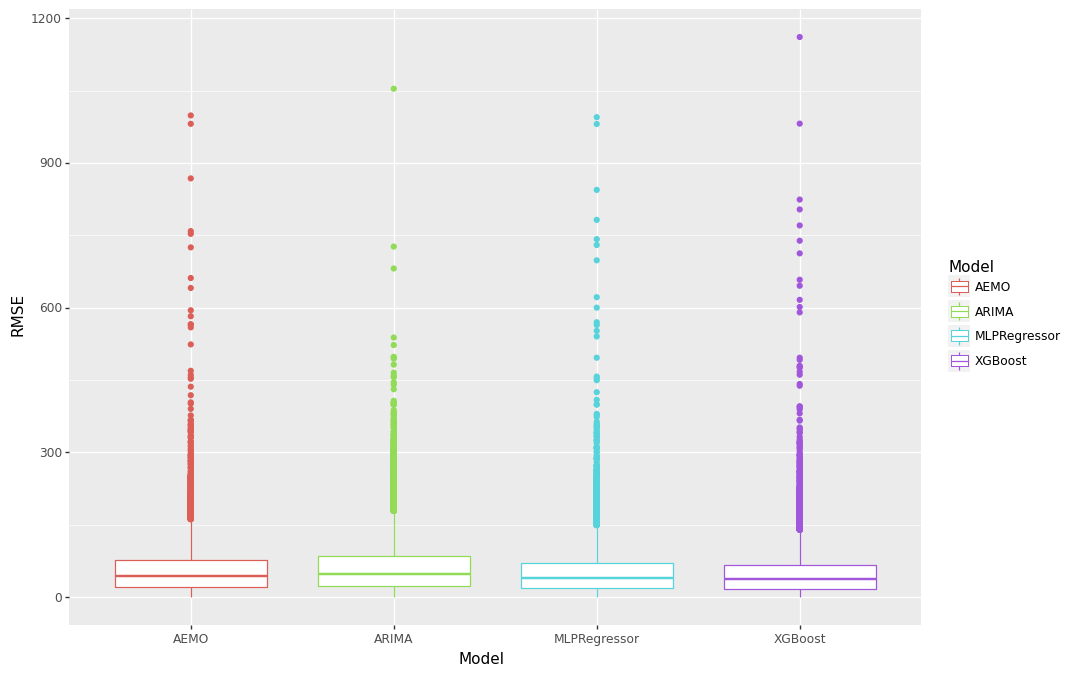
\includegraphics[width=140mm]{image16.png}
\caption{RMSE comparison of the prediction for different models}
\label{image16}
\end{figure}

The performance of the ARIMA(4,1,2) model was not as great as the
XGBoost, as it has a larger RMSE. One possible explanation for this is
due to the fact that time series only takes into account the past values
of a single attribute when modelling the future values of that same
value. As there are a multitude of factors that can influence
electricity demand, having a model that only considers one feature is
not ideal. In addition to the fact that the performance of the XGBoost
is superior to that of the time series, it was collectively agreed upon
that we would not further investigate other ARIMA, ARIMAX or SARIMA
models, as it does not meet our initial objective of building a model
that accounts for factors that are currently not included in the AEMO's
model. However, ARIMA is good at detecting outliers which should be used
for prediction of unusual events.

The performance of the MLPRegressor model was better than ARIMA as it
acts as a sliding window across the data to input 200 data points into
200 hidden nodes at a time resulting in not having historical
information to be able to detect outliers well compared to ARIMA.
However, MLPRegressor didn't perform as well as XGBoost Regressor as the
overall performance of the XGBoost Regressor model was greater than
other models (the AEMO's model ARIMA, LSTM and MLP Regressor) as it
offered the lowest RMSE. The reason is that XGBoost regressor offers
optimised implementation of gradient boosting which calculates residual
errors from the latest predictor and tries to fit the new predictor to
these residual errors. XGBoost includes a unique split-finding algorithm
to optimise trees, along with built-in regularisation that reduces
overfitting. It is scalable and very fast. This model is also easy to
tune with minimum parameters to tune and fast to re-train. For the
outliers, XGBoost Regressor performs worse than the ARIMA model as
XGBoost Regressor does not have information about history and trends
which caused by some unusual events (for example, due to bushfires,
COVID lockdown in 2020) to be able to predict outliers correctly.

Due to the limited outliers in the train dataset, we further investigate
by training data with the more outliers from 2012 onwards. We discovered
that the more outliers to train, the better the model as outliers are a
sparse dataset contributing to accuracy of predictions. Due to its
complexity and its ability to retain prior information in predicting
future values, our initial expectations were that the LSTM model would
have produced the lowest RMSE. Thus it was rather surprising that the
LSTM model had one of the worst performing outcomes out of all the
models tested. Whilst further work can be done to improve the
performance of the LSTM (further hyperparameter optimisation, more
epochs, and a grater lag etc.), it is unlikely that there would be
significant gain in predictability in the timeframe we had.

To visualise the performance of the models, we compared the RMSE for the
model, as well as for the outliers. Figure \ref{image19} Shows that
comparison, it clearly shows the benefit of the ARIMA for outlier
events, as well as the benefit of the XGBoost for normal day to day
operations.

\begin{figure}[H]
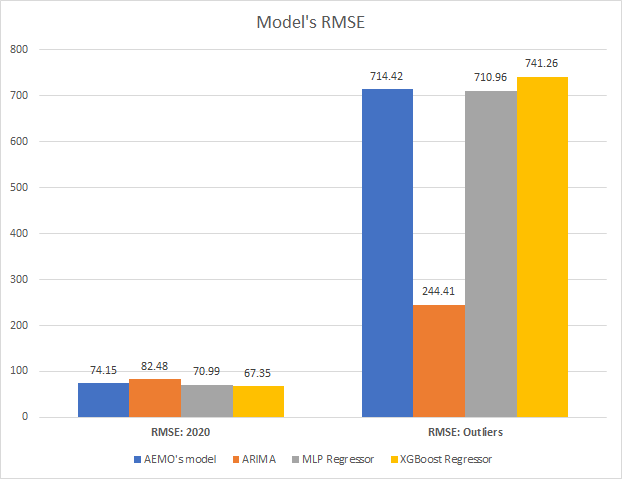
\includegraphics[width=140mm]{image19.png}
\caption{RMSE comparison of the prediction for all data and the outlier subset for the selected models}
\label{image19}
\end{figure}

In addition, to visualise the accuracy of each of the models we used a
binning techique to graph the difference between total demand and
predicted demand in bin sizes of 100, it was interesting to note, that
very few of the models wever got the predictions correct, and in fact
the most common values of diffeence where in the range of 100-200.
Figure \ref{bin} shows this.

\begin{figure}[H]
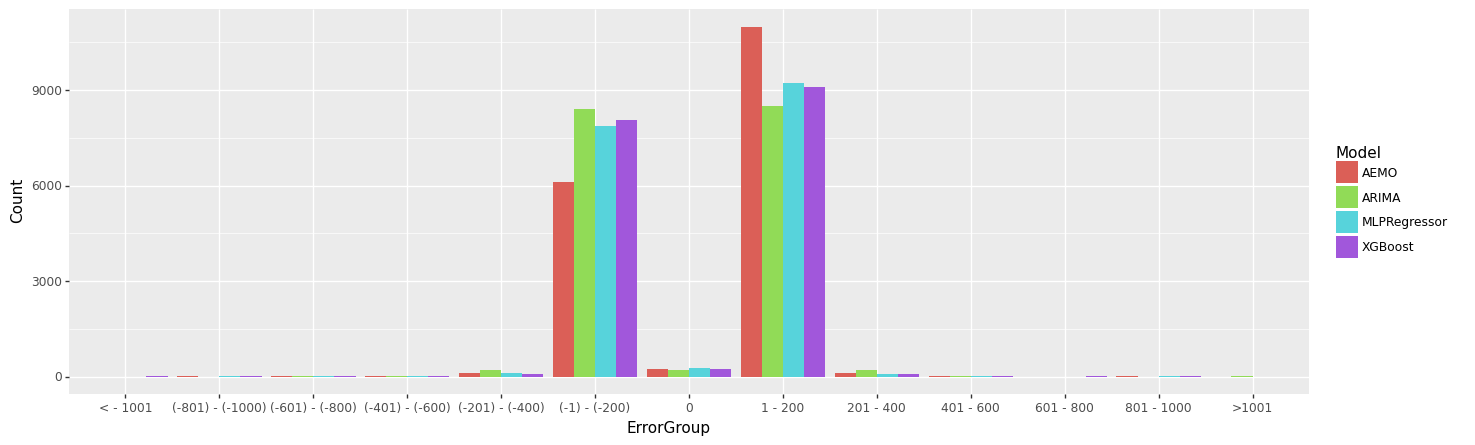
\includegraphics[width=140mm]{image34.png}
\caption{Comparison of binned values of total demand - predicted demand for each model}
\label{bin}
\end{figure}

Whilst our models where able to increase the accuracy of the both the
outliers and the overall model, it is important that the capability we
have created is easily able to be used. This capability is dependent on
several components, it requires the input of the temperature data, the
current forecast data, the public holiday data, as well as the PV data.
In the current modeling that the AEMO does, they have the forecast,
public holiday, and the temperature data. This means the only new data
that they need to build is the PV data. The AEMO only used the public
holiday data to differentiate between working day, and non working day,
we have used more granular categories to build a more accurate model.

The PV data was created by using a single 5.1kW system as the baseline,
this was then normalised to a per MW value. The total MW usage across
the state was then used to scale this up to current usage. The total MW
values are monthly based forecasts, and this data could be refreshed
each month, and used for future forecasts. The daily data is more
challenging to predict, whilst not in the scope of the project, we have
identified several ways this could be done. The theoretical amount of PV
data can be calculated from the lattitutde, longittude and the air mass
index at the time of the forecast. This data follows a similar curve to
that which has been seen by the single system. This theoretical maxim
would then be multiplied by a normalisation factor calculated by
comparing several days worth of forecasts. The PV data could be
predicted based on the BOMs UV data or similar, and a model built up and
compared to the current PV data. Alternative research by Maleki et
al.~provides a review of several other techniques if more precision is
required\cite{en10010134}.

The limits of the capability of our model is also the abillity to
predict the outlier days. The ARIMA model was the best at caluclating
the outliers, this is because for most of the extreme events where the
difference between forecast demand and the observerd total demand did
not coerrelate well with either temperature or PV data. Whilst they
nearly all occured on either extremely hot, or very cold days, there was
also many extrememly hot or very cold days that the model forecasted
accurately. We believe the reason for this is that the outlier evetns
where caused by other social phenomonens, or impactful events. For
instance the outliers on the 4th January 2020 was likely caused by the
bushfires and the failure of one of the electtical power stations,
similarily the outlier event on the 13th July 2020 was liekly caused by
COVID lockdown in Sydney. Our recomendation would be that in the event
of a large discrepnency between the XGBoost forecast and the observed
total demand, then changing to the arima model for a period of time
would be prefferable.

\hypertarget{conclusion-and-further-issues}{%
\chapter{Conclusion and Further
Issues}\label{conclusion-and-further-issues}}

The modeling that we have done shows that our system has the capability
of increasing the accuracy of AEMO's modeling. We have shown that the
use of PV data and by more granular categorisation of public holiday and
weekday data it is possible to build a more accurate model. The XGBoost
model that we generated was able to provide a 9.2\% increase in
performance when compared to the current AEMO's prediction.

When comparing between models, we had expected that the LSTM model would
be the most accurate, however due to the naivete of our model this did
not result in an accurate prediction of total demand. The MLPRegressor
model was only slightly worse than the final XGBoost model, this is to
be expected as they both rely on similar underpinning optimisations. The
ARIMA model was surprisingly accurate for the outlier events, this is
likely due to the fact that the lack of correlation between the data
sources used and outliers means that the previous values is a better
indicator of total value than other data observations.

For our model to be successfully implemented it requires AEMO to start
collecting PV data, and PV forecast data. It requires both the PV data
for a single system (or theoretical calculation) multiplied by the
current installed base. It is likely that as PV rollout continues across
the state, this will become an increasing factor in both detecting and
managing anomalous events in the future.

The best implementation of our model would be done with a parallel
implementation of both the ARIMA and the XGBoost model, whilst the
absolute difference between forecast demand and total demand was less
than 500 the XGBoost model should be used, however, when the absolute
difference moved outside of this value, then it should use the ARIMA
models output. Due to time constraints, we were unable to model the
duration of time to run the ARIMA model, however, it is likely that this
should only be for a period of a couple of hours. It should be noted
that attempting to use a less than absolute difference of 500 when end
up with an unstable oscillation between the models, hence further
research is required to accurately build this implementation.

It was also noted that whilst the PV Data does increase the accuracy of
the model, the outlier events do not strongly correlate with either PV,
temperature or public holiday data, it is likely that an additional data
set would be required to predict outlier events. During the process of
the project we identified that both COVID and bushfires where likely to
be the cause of outlier events.

As shown in the literature review as technologies have changed, so has
the need for the electrical industry to respond. The need for accurate
and timely forecasts of demand is becoming increasingly challenging.
Over the coming years energy storage devices such as large capacity
batteries and pumped hydro as energy storage will change the landscape
of energy demand forecasting. Future research should include identifying
and creating additional data sources in this area.

\bibliographystyle{elsarticle-num}
\bibliography{references}

\hypertarget{appendix}{%
\chapter*{Appendix}\label{appendix}}
\addcontentsline{toc}{chapter}{Appendix}

\hypertarget{glossary}{%
\section*{\texorpdfstring{\textbf{Glossary}}{Glossary}}\label{glossary}}
\addcontentsline{toc}{section}{\textbf{Glossary}}

\begin{table}[H]
\centering
\begin{tabular}{p{0.3\linewidth} | p{0.6\linewidth}} 
\hline\hline
\textbf{Item}               & \textbf{Description}                                                                                                      \\
\hline\hline
AEMO               & Australian Energy Market Operator                                                                                \\
VIF                & Variance inflation factor                                                                                        \\
RMSE               & Root Mean Square Error (We avoid RMSEP to avoid confusion)                                                       \\
PV                 & Photovoltaics                                                                                                    \\
MLPRegressor       & Multilayer Perceptron Regressor                                                                                  \\
LSTM               & Long Short-Term Memory                                                                                           \\
XGBoost            & XGBoost is a decision-tree-based ensemble Machine Learning algorithm                                             \\
ARIMA              & Autoregressive Integrated Moving Average                                                                         \\
EDA                & Exploratory Data Analysis                                                                                        \\
PowerBI            & Power BI is a business analytics service by Microsoft                                                            \\
NSW                & New South Wales                                                                                                  \\
NEM                & National Electricity Market                                                                                      \\
APVI               & Australian PV Institute                                                                                          \\
kWp                & kilowatts peak - peak power of a PV system or panel                                                              \\
NEMS               & National Electricity Market System                                                                               \\
HourMinute         & A variable for the combination of Hour and Minute of 24 Hours time                                               \\
DayName            & Name of the seven week days                                                                                      \\
Spot market        & Where financial instruments, such as commodities, currencies, and securities, are traded for immediate delivery  \\
Box-Jenkins method & A  Model is a mathematical model designed to forecast data ranges based on inputs from a specified time series   \\
AIC                & The Akaike information criterion                                                                                 \\
Adam               & Adaptive Moment Estimation                                                                                       \\
SGD                & Stochastic gradient descent                                                                                      \\
LBFGS              & Limited-memory Broyden-Fletcher-Goldfarb-Shanno Algorithm                                                        \\
SARIMA             & Seasonal Autoregressive Integrated Moving Average                                                                \\
ARIMAX             & Autoregressive–moving-average model with exogenous inputs                                                        \\
BOM                & Bureau of Meteorology                                                                                            \\
UV                 & Ultraviolet                                                                                                      \\
\hline\hline
\end{tabular}
\end{table}

\hypertarget{tables}{%
\section*{\texorpdfstring{\textbf{Tables}}{Tables}}\label{tables}}
\addcontentsline{toc}{section}{\textbf{Tables}}

\begin{table}[H]
\centering
\begin{tabular}{ll} 
\hline\hline
\textbf{VIF Factor} & \textbf{features}                 \\ 
\hline\hline
92.978786           & FORECASTDEMAND                    \\
104.845037          & YEAR                              \\
7.94458             & MONTH                             \\
4.179661            & DAY                               \\
6.746915            & HOUR                              \\
2.75231             & MINUTE                            \\
1.093466            & PUBLICHOLIDAYS                    \\
1.572454            & PVGeneration(MW)                  \\
1.074539            & HOURMINUTE\_14-30                 \\
1.080066            & HOURMINUTE\_16-30                 \\
1.12683             & HOURMINUTE\_18-0                  \\
1.118781            & HOURMINUTE\_18-30                 \\
1.134109            & HOURMINUTE\_19-0                  \\
1.107565            & HOURMINUTE\_2-0                   \\
1.118149            & HOURMINUTE\_2-30                  \\
1.132064            & HOURMINUTE\_20-0                  \\
1.116615            & HOURMINUTE\_20-30                 \\
1.138781            & HOURMINUTE\_21-0                  \\
1.081735            & HOURMINUTE\_9-0                   \\
1.100514            & HOURMINUTE\_9-30                  \\
1.999137            & DAY\_NAME\_Friday                 \\
2.02014             & DAY\_NAME\_Monday                 \\
2.079947            & DAY\_NAME\_Saturday               \\
2.138461            & DAY\_NAME\_Sunday                 \\
1.997267            & DAY\_NAME\_Thursday               \\
2.001941            & DAY\_NAME\_Tuesday                \\
3.391713            & SEASON\_autumn                    \\
3.18336             & SEASON\_summer                    \\
2.920135            & SEASON\_winter                    \\
1.052842            & TEMPERATURERANGES\_extremelyhigh  \\
1.117071            & TEMPERATURERANGES\_veryhigh       \\
1.486606            & TEMPERATURERANGES\_verylow        \\
\hline\hline
\end{tabular}
\label{VIF}
\end{table}

\hypertarget{additional-graphs}{%
\section*{\texorpdfstring{\textbf{Additional
graphs}}{Additional graphs}}\label{additional-graphs}}
\addcontentsline{toc}{section}{\textbf{Additional graphs}}

\begin{figure}[H]
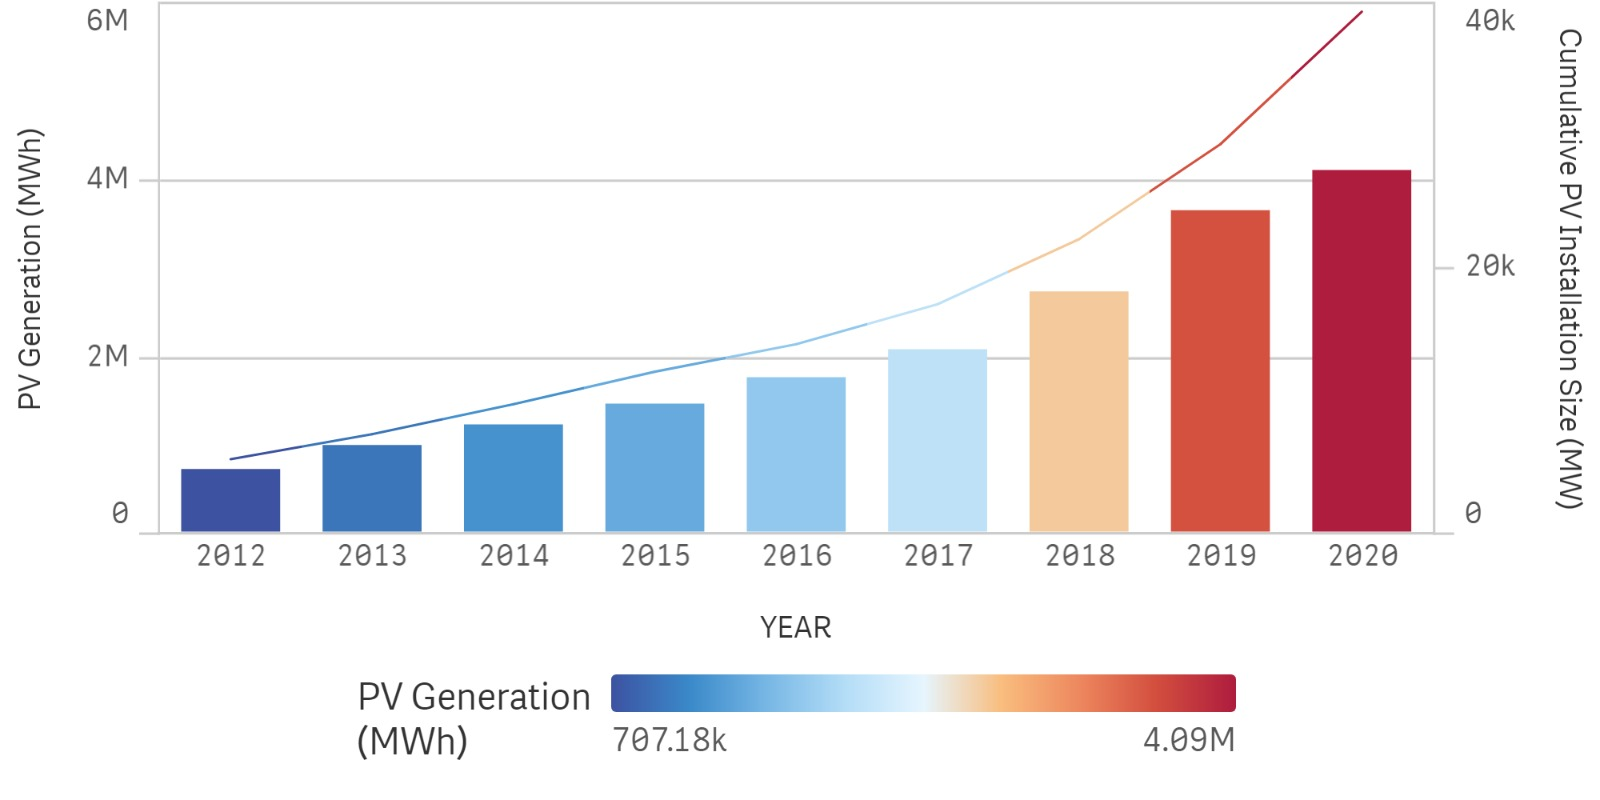
\includegraphics[width=140mm]{RFSolar.jpeg}
\caption{Expansion of the rooftop solar from 2012 to 2020 }
\label{RFSolar}
\end{figure}

\begin{figure}[H]
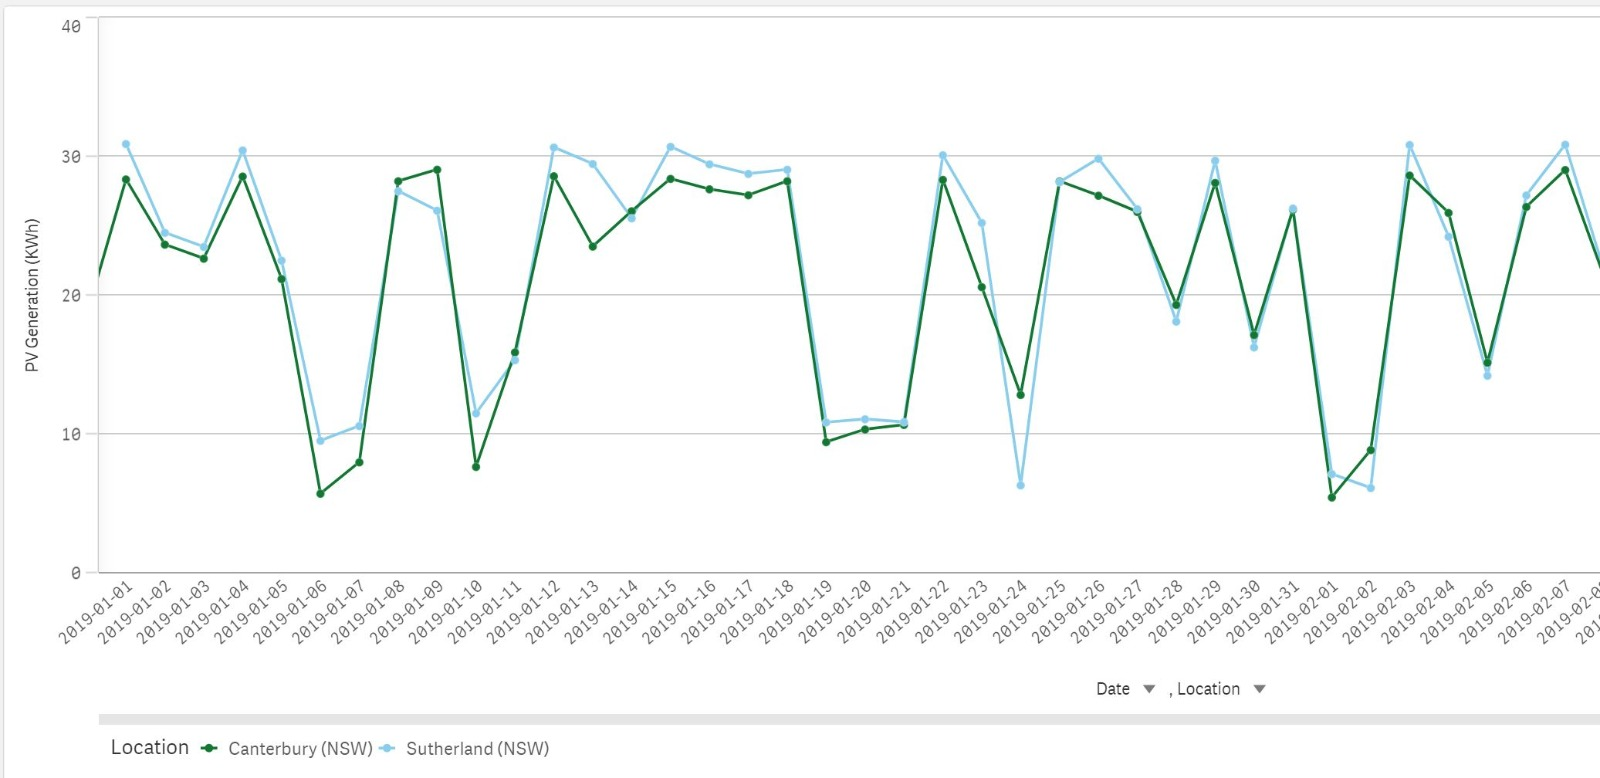
\includegraphics[width=140mm]{Cant.jpeg}
\caption{PV Performance comparison between Canterbury and Sutherland generated by single 5Kwp system }
\label{Cant}
\end{figure}

\begin{figure}[H]
\includegraphics[width=140mm]{XGBoost_Tune.jpeg}
\caption{Outlier prediction by XGBoost highlighting the error for the event on the 4th of January }
\label{XGTune}
\end{figure}







\end{document}

